\documentclass[report,gutter=10mm,fore-edge=10mm,uplatex,dvipdfmx]{jlreq}

\usepackage{lmodern}
\usepackage{amssymb,amsmath}
\usepackage{ifxetex,ifluatex}
\usepackage{actuarialsymbol}
\usepackage[]{natbib}
\RequirePackage{plautopatch}

% maru suji ① etc.
\usepackage{tikz}
\newcommand{\cir}[1]{\tikz[baseline]{%
\node[anchor=base, draw, circle, inner sep=0, minimum width=1.2em]{#1};}}

\usepackage{comment}

\begin{comment}

\ifnum0\ifxetex1\fi\ifluatex1\fi=0 % if pdftex
  \usepackage[T1]{fontenc}
  \usepackage[utf8]{inputenc}
  \usepackage{textcomp} % provide euro and other symbols
\else % if luatex or xetex
  \usepackage{unicode-math}
  \defaultfontfeatures{Scale=MatchLowercase}
  \defaultfontfeatures[\rmfamily]{Ligatures=TeX,Scale=1}
\fi
% Use upquote if available, for straight quotes in verbatim environments
\IfFileExists{upquote.sty}{\usepackage{upquote}}{}
\IfFileExists{microtype.sty}{% use microtype if available
  \usepackage[]{microtype}
  \UseMicrotypeSet[protrusion]{basicmath} % disable protrusion for tt fonts
}{}
\makeatletter
\@ifundefined{KOMAClassName}{% if non-KOMA class
  \IfFileExists{parskip.sty}{%
    \usepackage{parskip}
  }{% else
    \setlength{\parindent}{0pt}
    \setlength{\parskip}{6pt plus 2pt minus 1pt}}
}{% if KOMA class
  \KOMAoptions{parskip=half}}
\makeatother
\usepackage{xcolor}
\IfFileExists{xurl.sty}{\usepackage{xurl}}{} % add URL line breaks if available
\IfFileExists{bookmark.sty}{\usepackage{bookmark}}{\usepackage{hyperref}}
\hypersetup{
  hidelinks,
  pdfcreator={LaTeX via pandoc}}
\urlstyle{same} % disable monospaced font for URLs
\usepackage{longtable,booktabs}
% Correct order of tables after \paragraph or \subparagraph
\usepackage{etoolbox}
\makeatletter
\patchcmd\longtable{\par}{\if@noskipsec\mbox{}\fi\par}{}{}
\makeatother
% Allow footnotes in longtable head/foot
\IfFileExists{footnotehyper.sty}{\usepackage{footnotehyper}}{\usepackage{footnote}}

\end{comment}
%\makesavenoteenv{longtable}
\setlength{\emergencystretch}{3em} % prevent overfull lines
\providecommand{\tightlist}{%
  \setlength{\itemsep}{0pt}\setlength{\parskip}{0pt}}
\setcounter{secnumdepth}{-\maxdimen} % remove section numbering

\author{kazuyoshi}
\date{}

\newcommand{\problem}[1]{\subsubsection{#1}\setcounter{equation}{0}}
%\newcommand{\answer}[1]{\subsubsection{#1}}
\newcommand{\answer}[1]{\subsubsection{解答}}

%Pdf%\newcommand{\wakumaru}[1]{\framebox[3zw]{#1}}
\newcommand{\wakumaru}[1]{#1}






\begin{document}

\chapter{生保 2 第 1章-生命保険会計}

\section{1.1
生命保険会計の意義と特徴}

\problem{H30 生保2問題 3(1)①、H27 生保2問題 2(1) 、H18生保2問題 1(6)、
H14 生保2問題 2(1)①、H8 生保2問題 3(2)①、
H1生保2問題2(1)}

「生命保険会計の意義」および「生命保険会計の特徴(保険期間の超長期性から生じる特徴、群団性から生じる特徴、保険料構成要素の多様性等から生じる特徴)」について、簡潔に説明しなさい。

\answer{解答}

\paragraph{<意義>}

\begin{itemize}
\tightlist
\item
  生命保険会計とは、

  \begin{itemize}
  \tightlist
  \item
    生命保険会社の支払能力の状況、あるいは
  \item
    活動の実態等を
  \item
    金銭で評価し、会計の言葉で表現すること。
  \end{itemize}
\item
  一般会社と同じ点, 一般の企業会計

  \begin{itemize}
  \tightlist
  \item
    会社法および企業会計原則等に則った会計処理を行う
  \item
    「債権者および投資家の保護」に力点が置かれているが、
  \end{itemize}
\item
  特別の規定 (保険業法に存在), 生命保険会計

  \begin{itemize}
  \tightlist
  \item
    契約の全期間にわたり契約者保護が確実に遂行されるよう

    \begin{itemize}
    \tightlist
    \item
      契約者保護の観点から
    \end{itemize}
  \item
    生命保険会社の「支払能力確保」を重視した会計を指向。

    \begin{itemize}
    \tightlist
    \item
      生命保険会社の健全化を図るため
    \end{itemize}
  \end{itemize}
\item
  国際的な傾向として、

  \begin{itemize}
  \tightlist
  \item
    財務会計として一般企業と同じ尺度での比較が求められている
  \item
    日本では、保険業法による会計が唯一の法定会計。
  \end{itemize}
\item
  保険業法による会計だけで生命保険会社の情報を十分に表現できるものではない

  \begin{itemize}
  \tightlist
  \item
    業法会計では、保険販売の成果は超長期に亘って利益計上されるなど
  \end{itemize}
\end{itemize}

\paragraph{<特徴>}

\begin{itemize}
\tightlist
\item
  保険期間の超長期性

  \begin{itemize}
  \tightlist
  \item
    生命保険契約は契約の全期間を通じて生じる
  \item
    一定の偶発事故に対して保険給付の支払いを約し、
  \item
    その契約期間は超長期。

    \begin{itemize}
    \tightlist
    \item
      そのため、生命保険会社は超長期に亘って適正な支払能力の確保が必要。
    \item
      この点から資産評価の保守性と支払準備のための準備金の充実という特性が生じる。

      \begin{itemize}
      \tightlist
      \item
        (たとえば、資産評価を清算価値とすることや、危険準備金・追加責任準備金を積み立てるなど)
      \end{itemize}
    \end{itemize}
  \item
    支払能力の確保と期間損益の把握は表裏の関係

    \begin{itemize}
    \tightlist
    \item
      支払能力の評価により期間損益の評価(利益)も異なる。
    \item
      真の利益は群団の消滅まで確定しない。
    \end{itemize}
  \end{itemize}
\item
  群団性

  \begin{itemize}
  \tightlist
  \item
    保険制度は大数の法則を前提としており、
  \item
    目的毎に一定の群団を設定し、
  \item
    群団間の公平性を図りつつ支払能力の確保を図る。
  \item
    特に責任準備金の評価においてこの群団性を前提とした解釈をすることが必要。
  \item
    例えば、契約件数が極端に少ない場合、

    \begin{itemize}
    \tightlist
    \item
      群団として成立させることには無理があり、
    \item
      他の保険に統合する等の工夫が必要。
    \end{itemize}
  \item
    事業費は契約初年度と次年度以降で水準が大きく異なるため、

    \begin{itemize}
    \tightlist
    \item
      収益・費用の対応を目的とした会計では、

      \begin{itemize}
      \tightlist
      \item
        新契約の世代毎に群団を分け、

          チルメル式等の考慮を行うこともありうるが、
      \item
        世代をまたいだ1つの群団として維持・管理し、

          世代間で相互扶助を行いながら支払能力の確保を図るという解釈もありうる。
      \end{itemize}
    \end{itemize}
  \end{itemize}
\item
  保険料の構成要素の多様性

  \begin{itemize}
  \tightlist
  \item
    保険料計算基礎には複数の要素

    \begin{itemize}
    \tightlist
    \item
      (予定利率、予定死亡率、予定事業費率等)があり、
    \item
      平準保険料方式を採用。
    \end{itemize}
  \item
    この前提から、収益である保険料を費用に対応させる方法は、その目的に応じ様々考えられるが、

    \begin{itemize}
    \tightlist
    \item
      普遍的に正しい方法があるわけではない。
    \end{itemize}
  \end{itemize}
\end{itemize}

\subparagraph{まとめ}

\begin{itemize}
\tightlist
\item
  保険契約の\textbf{長期性}、\textbf{支払能力の確保}等の特性を考慮したうえで、\textbf{毎期の利益をどう評価するか}は極めて重要な課題。これには、\textbf{保険数理の技法が強く要請される}が、これはアクチュアリーの大きな職務の一つである。
\end{itemize}

\problem{H28 生保2問題1(1)}

生命保険会計に関する以下の(1)~(5)の文章について、下線部分が正しい場合は○を記入し、下線部分が誤っている場合は×を記入するとともに正しい内容に改めなさい。

\begin{enumerate} [(1)]
 \item  損益計算書の保険金勘定には、\underline{発生}主義により支払額を計上する
 \item  保険料が一括払いにより払い込まれた場合、翌事業年度に充当されるべき保険料相当額を、当事業年度末において\underline{未経過保険料}として積み立てる。
 \item  保険事故が発生した契約において、死亡保険金が未払いの状態で同保険金にかかる支払備金が計上される場合、当該契約の死亡保険金額は事業年度末の保有契約高に計上\underline{される}。
 \item 
 次の契約において、事業年度末直前に解約の申し出があり解約処理を行ったが、事業年度末現在、解約返戻金は未払いの状態であった。このとき、支払備金に計上する金額は、\underline{1,200} 千円である。\\ 
       契約:死亡保険金 10,000 千円、解約返戻金 1,500 千円、契約者貸付金 300 千円
 \item  前納契約が消滅した場合の前納残高の返還金は、「\underline{保険料}」勘定に計上される。
\end{enumerate}
]

\answer{解答}

\begin{longtable}[]{@{}lll@{}}
\toprule
設問 & ○ か × かを記入 & × の場合に正しい内容を記入\tabularnewline
\midrule
\endhead
① & × & 現金\tabularnewline
② & ○ &\tabularnewline
③ & × & されない\tabularnewline
④ & × & 1,500千円\tabularnewline
⑤ & × & その他返戻金\tabularnewline
\bottomrule
\end{longtable}

\problem{H10 生保2問題1(1)}

次の①~⑤の文章のうち、正しいものに○、誤っているものに×をつけよ。

\begin{enumerate} [(1)]
\item 責任準備金の「限度積立」にかかる実際の計算は、年度末有効契約に対して払込期日の到来した保険料につき、すべて収入があったものとして計算し、そこから未収保険料中の保険料積立金を差し引いて算出する。
\item 次年度以降の保険料を前納した場合、その前納保険料に対して、決算時に損益計算書に計上する責任準備金繰入額は、前納保険料残高の利息による増加分から当事業年度中に充当した保険料を差し引いた額に等しい。
\item 下記のような契約が事業年度末直前において解約の申し出があり、解約処理を行ったが、事業年度末現在、解約返戻金は未払いの状態であったので、解約返戻金から契約者貸付金を差し引いた1,100円を支払備金に計上した。 

死亡保険金 10,000 千円、解約返戻金 1,200円、契約者貸付金 100 千円
\item 契約変更の場合の経理処理で、契約者貸付金のない場合の払済保険への変更や、契約転換で被転換契約の責任準備金のうち転換後契約の責任準備金に充当する部分については、経理処理を行わない。
\item 決算では収入保険料と保有契約および責任準備金の 3 者は相互に完全に対応していなければならない。
\end{enumerate}

\answer{解答}

(1)×、

 技術上の問題から, 年度末有効契約に対して

\begin{itemize}
\tightlist
\item
  一応払込期日の到来した保険料につきすべて収入のあつたものとして計算し、
\item
  そこから未収保険料中の保険料積立金および\textbf{未経過保険料相当分}を各々差し引いて算出する。
\item
  ただし、決算時から猶予期間末までの期間内に\textbf{保険料の収入が見込まれない契約}についての当該期間に対する\textbf{危険保険料相当額}は、保険料の収入が見込まれない契約からも死亡保険金等の請求だけはあると考えて、これを\textbf{加える}こととしている。
\end{itemize}

(2)○、 

(3)×、

支払備金は、\textbf{契約者貸付がある場合}でも、\textbf{貸付金を控除する前の金額を計上する}こととなっているから、支払備金としては解約返戻金として1,200千円を計上することになる。

④○、 

⑤○


\problem{H8 生保2問題1(1)}

保険料の計上を現金主義としている理由について説明せよ。

\answer{解答}

保険料の計上を、入金を手がかりとして行おうとする意図は、

\begin{itemize}
\tightlist
\item
  保険料の \textbf{債権としての位置付け} によっている。
\item
  つまり、保険料の支払は \textbf{契約者の自由意志} に基づくものであり、
\item
  未収保険料は保険会社の \textbf{確定債権とはいえない}
  と考えられるため、
\item
  払込期日の到来等により収益として計上することは、\textbf{保守主義の原則}
  の観点から妥当ではないと考えられるものである。
\end{itemize}


\problem{H2 生保2問題2(2)}

保険料計上における期間損益の把握と責任準備金の関係について、前納の場合を例にとり簡単に説明せよ,


\answer{解答}

2.前納とは次期以降の保険料を前払いする制度であり、\textbf{保険料収入}としては当期分も次期以降分も、\textbf{すべて当年度収益}として計上する。このままでは当期の収益が過大となるため、次期以降にかかる部分を\textbf{未経過保険料}として\textbf{責任準備金}に積み立てることにより損益の調整を行っている。
なお、その後の毎年の損益計算は、保険料充当は特段の経理処理を行わず、\textbf{前納保険料残高の洗い替え}により自動的に一回分保険料が収益計上されたと同じ効果を生じさせることとしている。

\subsection{限度積立}

\problem{H19 生保2問題
1(1)}

保険料と責任準備金に関し、以下の空欄を埋めよ。

\begin{itemize}
\tightlist
\item
  日本の生命保険会計において保険料の計上は①主義によっており、②は計上しない。
\item
  保険料に対応し、責任準備金の積立ても保険料の入金を限度として行っている。これを責任準備金の「③」と呼んでいる。実務での計算は一般的に年度末有効契約に対して一応④の到来した保険料につきすべて収入のあったものとして責任準備金を計算し、そこから②中の保険料積立金及び未経過保険料相当分を各々差し引いて算出する。ただし、決算時から猶予期間末までの期間内に保険料の収入が見込まれない契約についての当該期間に対する⑤相当額を加算する。
\end{itemize}

\answer{解答}

① 現金, ② 未収保険料, ③ 限度積立, ④ 払込期日, ⑤ 危険保険料

\begin{center}\rule{0.5\linewidth}{0.5pt}\end{center}

\problem{H12 生保2問題
1(1)}

次の①~⑤を適当な語句で埋めよ

いわゆる責任準備金の「限度積立」の一般的な計算は以下のとおりである。責任準備金は、年度末①に対して②の到来した保険料についてはすべて収入のあったものとして計算し、そこから③中の保険料積立金および未経過保険料相当分を各々差し引いて算出する。ただし、決算時から④末までの期間内に保険料の収入が見込まれない契約についての当該期間に対する⑤相当額は、保険料の収入が見込まれない契約からも死亡保金請求はあると考えて、これを加えることとしている。


\answer{解答}

①有効契約(保有契約等も可), ②払込期日, ③未収保険料, ④猶予期間,
⑤危険保険料

\subsection{支払備金}

\problem{H14 生保2問題
1(1)}

次の①~⑤を適当な語句で埋めよ。
生命保険会社における費用の計上基準は①主義である。実務上、期中における保険契約上の給付について、支払時においては②主義により処理するが、事業年度末において③勘定を用い①主義による処理に修正する。
保険業法で③として、次の 2 種類の積立を要求している。

\begin{itemize}
\tightlist
\item
  ④が発生しているが、決算期においてまだ支出として計上していない保険金等
\item
  支払事由の発生の⑤を受けていないが、支払事由が既に発生したと認められる保険金等
\end{itemize}


\answer{解答}

①発生, ②現金, ③支払備金, ④支払義務, ⑤報告

\problem{H18 生保2問題 1(5)、H8 生保2問題 1(3)、H4 生保2問題
1(2)}

支払備金について簡潔に説明せよ。

\answer{解答}

保険金等で、
\begin{enumerate} [A.]
 \item 支払義務が発生しているが、決算期においてまだ支出として計上していない保険金等(施行規則第73条)
\item 決算期においてまだ支払事由の発生の報告を受けていないが、支払事由が既に発生したと認められる保険金等(既発生未報告備金:IBNR備金)(施行規則第72条,
 業法第117条) がある場合、「支払備金」として積み立てなければならない。
\end{enumerate}

生命保険会計における費用の計上基準は発生主義である。実務上は、期中の保険契約上の保険金等を、その支払時に現金主義により処理し、事業年度末において「支払備金」勘定を用いることによって発生主義による処理に修正する。

保険業法施行規則第73条は、保険会社が毎決算期に支払備金として、「保険契約に基づいて支払業務が発生した保険金等(当該支払業務に係る訴訟が係属しているものを含む。)のうち、決算期において、まだ支出として計上していないものがある場合は、当該支払のために必要な金額」および「第72条に規定する保険金等についてその支払のために必要なものとして計算した金額」を積み立てなければならないことを規定している。保険業法施行規則第72条は、保険業法第117条で支払備金を積み立てなければならない「保険契約に基づいて支払業務が発生したものに準ずるもの」について、「保険金、返戻金その他の給付金であって、決算期において、保険会社が、まだ支払事由の発生の報告を受けていないが保険契約に規定する支払事由が既に発生したと認められるもの(いわゆるIBNR)」と規定している。

保険契約消滅事由が発生したにもかかわらず、何らかの事情で事業年度末に当該事由に対する支払が行われていない場合には、会社はその金額を「支払備金」に計上しなければならない。期中の保険契約上の給付は、支払時に現金主義で処理されるが、事業年度末に「支払備金」勘定を用いることにより発生主義に修正されることになる。

\problem{H27 生保2問題
1(6)}

ある生命保険会社の X 事業年度末における既発生未報告支払備金(IBNR
備金)積立額を下表に基づき計算し、解答欄に記入しなさい。ただし、計算過程においては端数処理を行わず、解答においては百万円未満を四捨五入して百万円単位とする。なお、記載のない項目は考慮する必要はない。

(単位:百万円)

\begin{longtable}[]{@{}lllllll@{}}
\toprule
事業年度 & 保険金等の収入額 & 保険料等の支払額 & 保有契約高 & IBNR
備金積立所要額 & IBNR 備金積立額 &\tabularnewline
\midrule
\endhead
X & 480,000 & 250,000 & 40,000,000 & & &\tabularnewline
X-1 & 420,000 & 240,000 & 36,000,000 & 4,536 & 4,436 &\tabularnewline
X-2 & 390,000 & 230,000 & 35,000,000 & 4,186 & 4,357 &\tabularnewline
X-3 & 360,000 & 225,000 & 30,000,000 & 4,140 & 4,251 &\tabularnewline
\bottomrule
\end{longtable}

(※)表中の「保有契約高」、「IBNR 備金積立所要額」 および「IBNR
備金積立額」は、事業年度末における数値

\answer{解答}

4,625 百万円 ・X-1年度分:4,536×250,000/240,000=4,725
・X-2年度分:4,186×250,000/230,000=4,550
・X-3年度分:4,140×250,000/225,000=4,600
⇒(4,725+4,550+4,600)/3=4,625 百万円

当年度IBNR備金積立額は、以下3年分の平均として求める

\begin{itemize}
\tightlist
\item
  前年度末 IBNR 備金所要額×当年度支払額÷前年度支払額
\item
  前々年度末 IBNR 備金所要額×当年度支払額÷前々年度支払額
\item
  前々々年度末 IBNR 備金所要額×当年度支払額÷前々々年度支払額
\end{itemize}

\section{1.3
保険契約準備金}

\problem{H18 生保2問題1(2)改題}\footnote{6項の一の二が追加されているのみ}

保険業法施行規則第六十九条(生命保険会社の責任準備金)について、以下の空欄を埋めよ。

第六十九条(生命保険会社の責任準備金)

生命保険会社は、毎決算期において、次の各号に掲げる区分に応じ、当該決算期以前に収入した①を基礎として、当該各号に掲げる金額を法第四条第二項第四号に掲げる書類に記載された方法に従って計算し、責任準備金として積み立てなければならない。

一 ②\\
保険契約に基づく将来の債務の履行に備えるため、③に基づき計算した金額(第二号の二の払戻積立金として積み立てる金額を除く。)

二 ④\\
未経過期間(保険契約に定めた保険期間のうち、決算期において、まだ経過していない期間をいう。次条及び第二百十一条の四十六において同じ。)に対応する責任に相当する額として計算した金額(次号の払戻積立金として積み立てる金額を除く。)

二の二 払戻積立金(省略) 

三 危険準備金(省略) 

2~5 (省略) 

6 第一項第三号の危険準備金は、次に掲げるものに区分して積み立てなければならない。

一  第八十七条第一号に掲げる保険リスクに備える危険準備金 

一の二 同条第一号の二に掲げる第三分野保険に備える危険準備金 

二 同条第二号に掲げる予定利率リスクに備える危険準備金 

三 同条第二号の二に掲げる⑤に備える危険準備金 

7(省略)


\answer{解答}

①保険料, ②保険料積立金, ③保険数理, ④未経過保険料, ⑤最低保証リスク

\problem{H25 生保2問題 2(1)改題、H20 生保2問題 3(2)①②、H16
生保2問題 4(1)② 、H12 生保2問題
2(1)①}

生命保険の責任準備金の評価において、計算基礎率をロック・インとする方式とロック・インとしない方式(ロック・フリー方式)を比較した場合のロック・インとする方式のメリットおよびデメリットについて、簡潔に説明しなさい。

\answer{解答}

\paragraph{ロック・イン方式のメリット}

\subparagraph{利益の安定性}

責任準備金評価基礎率の遡及変更は、責任準備金の大幅な変更をもたらす場合がある。特に、利率引き下げの場合は大幅な負債の増加をもたらす。責任準備金の評価にあたっては支払能力の確保だけではなく、適正な利益の算出の目的も意識する必要があり、利益に与える影響の変動が少ないロック・イン方式のほうが望ましい面がある。

\subparagraph{契約者配当の安定性}

利益の変動が少ないことにより、契約者配当を、計画的・安定的に行える面がある。

\paragraph{ロック・イン方式のデメリット}

\subparagraph{金利低下局面等でのソルベンシーの確保}

契約時の評価基礎率を使用し続けることから、金利低下局面では、契約時の高い利率を用いて責任準備金を少なめに評価することがあり、支払能力確保の面で問題となる場合がある。

\subparagraph{金利上昇局面等でのサープラスの過小評価}

金利低下局面とは逆に、金利上昇局面では、債券を時価評価する場合、サープラスが過小に評価される欠点がある。

\subparagraph{標準利率・予定利率の設定方法}

標準責任準備金制度においては、標準利率が足元の市場金利とマッチせずに低い水準となっている場合、保険料計算用の予定利率を直近の市場金利に合わせると、標準責任準備金積増が発生することがある。

\subparagraph{標準基礎率の設定方法}

仮に、業界共通の経験率の蓄積が乏しい商品に対して標準基礎率を設定しようとした場合、各社がロック・フリー方式の基礎率を設定するよりも困難な場合がある。

\paragraph{ロック・フリー方式のメリット}

\subparagraph{資産評価と整合的}

バランスシート全体を市場整合的なものとした場合、資産と負債の評価が整合的となる。

\paragraph{ロック・フリー方式のデメリット}

\subparagraph{利益が不安定}

責任準備金評価基礎率の遡及変更は、責任準備金の大幅変更をもたらす場合、単年度の利益が不安定となる。

\subparagraph{契約者配当が不安定}

例えば、逆ざや契約等について責任準備金の変更額を積み増そうとする場合、当該保険群団の剰余だけでは不足するため、保険会社が過去蓄積してきた内部留保を充当せざるを得ず、当該保険群団以外の保険群団に配当還元の減少等の影響を及ぼし、契約間の衡平性を阻害することが考えられる。

\subparagraph{実務負荷}

フォーミュラ計算が可能なロック・イン方式とは異なり、実務負荷が大きい。

その他、予定利率以外の基礎率(予定死亡率・予定事業費率等)において、同様のメリット・デメリットが想定される。

\begin{center}\rule{0.5\linewidth}{0.5pt}\end{center}

\problem{H17 生保2問題
1(2)改題}

平成 8 年・大蔵省告示第 48
号に規定されている予定利率(標準利率)の水準の設定について、以下の空欄を適切な語句または数値で埋めよ。④については計算過程も記載せよ。

<平成 11 年 4 月 1
日以降の標準利率の水準の設定の概要\textbf{(平準払保険の場合)}> 毎年
10 月 1 日を基準日として、基準日の属する月の前月から過去①年間または過去
10 年間に発行された利付国庫債券(10
年)の応募者利回りのそれぞれの平均値のいずれか②い方の値を下表に掲げる対象利率に区分して、それぞれの数値に安全率係数を乗じて得られた数値の合計値(基準利率)が、基準日時点で適用されている予定利率と比較して③\%以上乖離している場合には、基準利率に最も近い
0.25%の整数倍の利率(基準利率が 0.25%の整数倍の利率と
0.125%乖離している場合は、基準利率を超えず、かつ、基準利率に最も近い
0.25%の整数倍の利率とする。)を予定利率とし、基準日の翌年の 4 月 1
日以降締結する保険契約に適用する。

\begin{longtable}[]{@{}ll@{}}
\toprule
対象利率 & 安全率係数\tabularnewline
\midrule
\endhead
0%を超え、1.0%以下の部分 & 0.9\tabularnewline
1.0%を超え、2.0%以下の部分 & 0.75\tabularnewline
2.0%を超え、\textbf{4.0%}以下の部分 & 0.5\tabularnewline
\textbf{4.0%}を超える部分 & 0.25\tabularnewline
\bottomrule
\end{longtable}

<標準利率の水準の計算> 平成 11 年以降のある年の 4 月 1
日時点で適用されている標準利率を
1.50%とする。同年の基準日の属する月の前月から過去に
①年間の利付国庫債券(10 年)の応募者利回りの平均値が 2.90\%、過去 10
年間の応募者利回りの平均値が 4.25%とすると、その翌年の 4 月 1
日以降締結する保険契約の標準利率の水準は④\%となる。
※上記\textbf{強調部}が現行規制との整合のため修正した箇所

\answer{解答}

①3 ②低 ③0.5 ④1×0.9+1×O.75+0.9×0.5=2.10(1.50と0.5以上乖離)→2.0%


\problem{H15 生保1問題
4(2)①}

標準責任準備金計算用の予定利率の設定ルールについて簡潔に説明せよ。


\answer{解答}

標準利率に関する設定ルールは、平成8年2月29日付大蔵省告示第48号に規定されている。概要は以下の通りである。

\begin{itemize}
\tightlist
\item
  平成11年3月31日までに締結する保険契約 2.75%
\item
  平成11年4月1日以降締結する保険契約 2.00%
\end{itemize}
  ただし、平成11年4月1日以降毎年10月1日を基準日として、次の計算をする。
\begin{enumerate}[ (A)]
\item 基準日の属する前日から過去3年間に発行された利付国債(10年)の応募者利回りの平均値、又は基準日の属する月の前月から過去10年間に発行された利付国債(10年)の応募者利回りの平均値を計算し、いずれか低いものを対象利率とする
\item その対象利率を利率ごとに区分し、各区分について安全係数を乗じた値を合算した利率を計算する。これを基準利率という。
\item 基準利率が基準日時点で適用されている標準利率と比較して0.5%以上乖離している場合には、基準利率に最も近い0.25%の整数倍の利率を標準利率とし、基準日の翌年の4月1日以降締結する保険契約に適用する。
\end{enumerate}

\begin{center}\rule{0.5\linewidth}{0.5pt}\end{center}

\problem{H15 生保2問題 1(1)、H10 生保2問題
1(2)}

標準責任準備金の対象外の契約に関して以下の空欄を埋めよ。

\begin{tabularx}{\linewidth}{|X|X|}
 \hline
対象外の契約 & 積み立てるべき金額 \\ \hline
\begin{itemize}
 \item 責任準備金が①に属する財産の価額により変動する保険契約 
\end{itemize}
&   ①の収支残 \\ \hline
\begin{itemize}
 \item   ②及び払戻積立金を積み立てない保険契約
\item
  責任準備金・保険料の計算基礎を変更できる旨、約款に規定している契約
\item
  保険業法第2条第5項第1号に掲げる保険に係る保険契約
\item
  保険期間③年以下の保険契約
\item
  ④をもって保険金、返戻金その他の給付金の額を表示する保険契約
\item
  平成8年3月 31 日以前に締結された契約
\end{itemize} & 保険料及び責任準備金の算出方法書で認可された予定利率及び予定死亡率その他保険事故を基礎として⑤により計算した金額
\\ \hline
\end{tabularx}

\answer{解答}

①特別勘定, ②保険料積立金, ③1, ④外国通貨, ⑤平準純保険料式

\begin{center}\rule{0.5\linewidth}{0.5pt}\end{center}

\problem{H30 生保2問題 1(1)、H21 生保2問題
1(1)}

標準責任準備金の対象外契約(平成 17 年 4 月 1
日以降に締結する保険契約)に関し、以下の①~⑤の空欄に当てはまる最も適切な語句または数字を記入しなさい。

\begin{itemize}
\tightlist
\item
  責任準備金が特別勘定に属する財産の価額により変動する保険契約であって、保険金等の額を
\item
  ①していない保険契約
\item
  ②及び払戻積立金を積み立てない保険契約
\item
  ③において、保険会社が責任準備金及び保険料の計算の基礎となる予定利率を変更できる旨を約してある保険契約(③において、当該保険契約の締結時の標準責任準備金の計算の基礎となるべき予定利率を超える利率を①している保険契約を除く。)
\item
  保険期間が④年以下の保険契約(注)
 \item ⑤をもって保険金、返戻金その他給付金の額を表示する保険契約
\end{itemize}

(注)積立勘定を設置して、保険期間の満了後満期返戻金を支払う旨を約した保険契約に係る責任準備金の金額に相当する財産の全部又は一部をその他の財産と分別して運用している保険契約については、保険期間が
10 年以下の保険契約


\answer{解答}

① 最低保証 ② 保険料積立金 ③ 保険約款 ④ 1 ⑤ 外国通貨

\problem{H11 生保2問題
1(1)}

次の①~⑤について、以下の A~D のうち当てはまる記号を答えよ。
\begin{enumerate} [(1)]
\item 定期保険(平成 8 年 4 月 1 日以降に締結した契約)
\item 終身保険(平成 8 年 3 月 31 日以前に締結した契約)
\item 変額保険(平成 8 年 4 月 1 日以降に締結した契約)
\item 団体信用生命保険(平成 8 年 4 月 1 日以降に締結した契約)
\item 新企業年金保険(平成 8 年 4 月 1日以降に締結した契約)
\end{enumerate} 

\begin{enumerate} [A ]
\item 標準責任準備金積立の対象であり、かつ、保険計理人の確認業務では将来収支分析を行う
\item 標準責任準備金積立の対象であり、かつ、保険計理人の確認業務では将来収支分析を行わなくともよい
\item 標準責任準備金積立の対象ではない、かつ、保険計理人の確認業務では将来収支分析を行う
\item 標準責任準備金積立の対象ではない、かつ、保険計理人の確認業務では将来収支分析を行わなくともよい
\end{enumerate}

\answer{解答}

① A、② C、③ D、④ D、⑤ D

\subsubsection{補足説明}

標準責任準備金積立対象外; 1.3.2.5 標準責任準備金対象外の契約等(1-35 〜 1-37)
\begin{itemize}
 \item 責任準備金が特別勘定の財産価額に依存(変額保険,変額年金,) かつ H17.4.1以降は最低保証していない: 積立金額 = 特別勘定の収支残
 \item 保険料積立金のない契約(団体定期保険, 団信も含まれる?): 積立金額 =平準純保険料式責任準備金, 標準基礎率を参考として適正に定めた予定利率・予定死亡率を基礎とする
 \item  (約款で) 責任準備金・保険料の計算基礎率( H13.7.1以降は予定利率,標準利率を超える利率を最低保証しているものは標準責任準備金の対象)を変更できる (新企業年金保険): 積立金額 =平準純保険料式責任準備金, 標準基礎率を参考として適正に定めた予定利率・予定死亡率を基礎とする
 \item (古い契約のみ) 予定死亡率以外の保険事故率 (優良体保険, 特定疾病保証保険); H12.4.1 (生命保険), H13.7.1 (第3分野)以降は標準責任準備金対象
 \item 保険期間1年以下; H12.3.31以前は5年
 \item 外国通貨
 \item 新保険業法施行前 (H.8.3.31以前)
\end{itemize}

将来収支分析(1号分析) (6-114〜); 施行規則80条, 実務基準第9条第2項. ロックイン方式の補完. 
実務基準第9条第5項 (1号分析の対象外)

\begin{itemize}
 \item 責任準備金を特別勘定の財産の価額に連動.かつ保険金額等の最低保証をしていない. 
 \item 保険料積立金を積み立てない
 \item 予定利率(古いもの; H13.7.1以前は基礎率)が固定されない
 \item その他標準責任準備金の計算の基礎となるべき係数の水準について必要な定めをすることが適当でない
\end{itemize}

\problem{2019 生保2問題 2(1)、H13 生保2問題 2(1)①、H8 生保2問題
3(1)}

標準責任準備金制度の目的および概要について説明せよ。

\answer{解答}

\paragraph{<目的>}

\begin{itemize}
\item
  1996 年 4 月に保険業法が改正
\item
  商品・価格の自由度がより高まり, 競争が促進されるようになった。
\item
  ただし、実質的な価格は事後に確定する保険の性格から,
  確固たる健全性確保の仕組みを併せて構築しておかなければ、却って消費者保護が図れなくなる可能性がある。
\item
  このため、保険会社の健全性を高め、支払能力を確保する視点から、長期の保険契約で内閣府令で定めるもの(標準責任準備金対象契約)については、
  内閣総理大臣(金融庁長官に委任)が,
  責任準備金の積立方法、計算基礎率水準について必要な定めを行うことができるとした、所謂「標準責任準備金」制度が設けられた。
\end{itemize}

\paragraph{<概要>}

\begin{itemize}
\tightlist
\item
  標準責任準備金制度とは、

  \begin{itemize}
  \tightlist
  \item
    内閣府令で定める「長期の保険契約」(標準責任準備金対象契約)について、
  \item
    金融庁長官が「責任準備金の積立方式及び予定死亡率その他の責任準備金の計算の基礎となるべき係数の水準」について必要な定めをすることができる、というもの。
  \end{itemize}
\item
  標準責任準備金の対象外の契約(平成 17 年 4 月 1
  日以降に締結する保険契約)

  \begin{itemize}
  \tightlist
  \item
    責任準備金が特別勘定に属する財産の価額により変動する保険契約であって、保険金等の額を最低保証していない保険契約
  \item
    保険料積立金及び払戻積立金を積み立てない保険契約、保険料積立金を計算しない保険契約
  \item
    保険約款において、保険会社が責任準備金及び保険料の計算の基礎となる予定利率を変更できる旨を約してある保険契約(保険約款において、当該保険契約の締結時の標準責任準備金の計算の基礎となるべき予定利率を超える利率を最低保証している保険契約を除く。)
  \item
    保険期間が1年以下の保険契約
  \item
    外国通貨をもって保険金、返戻金その他給付金の額を表示する保険契約
  \end{itemize}
\item
  責任準備金の積立方式及び予定死亡率その他の責任準備金の計算の基礎となるべき係数の水準

  \begin{itemize}
  \tightlist
  \item
    積立方式は、平準純保険料式
  \item
    予定死亡率は、公益社団法人日本アクチュアリー会が作成し、金融庁長官が検証したもの(生保標準生命表
    2018(死亡保険用)、生保標準生命表
    2007(年金開始後用)または第三分野標準生命表 2018)。
  \item
    ただし、当該予定死亡率以外の予定死亡率を責任準備金の計算の基礎として用いることが適当であると認められる保険契約を除く。
  \item
    予定利率は、保険料の払方や契約特性に応じて「第 1 号保険契約」、「第
    2 号保険契約」、「第 1 号保険契約及び第 2
    号保険契約以外の契約」に分けて設定された計算方式により定まる。
  \item
    第三分野商品の予定発生率、予定解約率など、共通の定めのない基礎率についても、制度の主旨に鑑み、保守的な設定が望まれる。
  \item
    契約時の評価基礎率を用いて評価するロックイン方式である。
  \item
    計算した保険料積立金の額が契約者価額を下回る場合には、契約者価額を保険料積立金とする。
  \item
    特別勘定を設けた保険契約であって、保険金等の額を最低保証している保険契約については、

    \begin{itemize}
    \tightlist
    \item
      一般勘定の責任準備金は、原則として、一般勘定における最低保証に係る保険金等の支出現価から一般勘定における最低保証に係る純保険料の収入現価を控除する標準的方式により算出した額とする。
    \item
      ただし、標準的方式により計算される責任準備金の債務履行を担保する水準と同等であることが認められる場合は、標準的方式に替えて、代替的方式を使用することができる。
    \item
      特別勘定の責任準備金は収支の残高とする。
    \end{itemize}
  \item
    生命保険会社の業務又は財産の状況および保険契約の特性等に照らし特別の事情がある場合には、標準責任準備金を下回る積み立てが認められている。ただし、この場合においても、保険料積立金及び払戻積立金の額は、保険数理に基づき、合理的かつ妥当なものでなければならない。
  \end{itemize}
\end{itemize}

\problem{H22 生保2問題
2(1)}

保険契約を再保険に付した場合の責任準備金の不積立てについて、関連する法令および「保険会社向けの総合的な監督指針」における記載も踏まえ、簡潔に説明しなさい。

\answer{解答}

\begin{itemize}
\tightlist
\item
  再保険に付した契約であっても、保険事故が発生した場合、保険金受取人からの請求に対して責任を負うのは元受保険会社であり、

  \begin{itemize}
  \tightlist
  \item
    再保険していることにより免責となるわけではない。
  \item
    受再会社が破綻した場合のことを考慮すれば、再保険に付した部分も含めて元受保険会社が責任準備金を積み立てることも考えられる。
  \item
    ただ、この場合、再保険方式によっては、元受保険会社に過度な負担を強いることになる。
  \end{itemize}
\item
  このため、保険業法施行規則において、

  \begin{itemize}
  \tightlist
  \item
    保険会社等に出再する場合は、健全な出再先への出再として、再保険を付した部分に相当する責任準備金を積み立てないことができるとされている。
  \end{itemize}
\item
  また、「保険会社向けの総合的な監督指針」においては、この取扱いの可否について、

  \begin{itemize}
  \tightlist
  \item
    当該再保険契約がリスクを将来にわたって確実に移転する性質のものであるかどうかや、
  \item
    当該再保険契約に係る再保険金等の回収の蓋然性が高いかどうかに着目して判断すべきであるとされ、

    \begin{itemize}
    \tightlist
    \item
      回収の蓋然性の評価にあたっては、少なくとも再保険契約を引き受けた保険会社又は外国保険業者の財務状況について、できる限り詳細に把握する必要がある、とされている。
    \end{itemize}
  \end{itemize}
\item
  生命保険の再保険として代表的なものに、

  \begin{itemize}
  \tightlist
  \item
    共同再保険方式や毎年の危険保険金部分を再保険する方式があるが、
  \item
    これらの再保険に付した契約における責任準備金については、

    \begin{itemize}
    \tightlist
    \item
      前者の場合は、保険料、保険金等の全ての契約者との金銭を再保険割合に応じて分かち合うことになるため、

      \begin{itemize}
      \tightlist
      \item
        責任準備金も元受会社と再保険会社で再保険割合に応じて積み立てなければ、収支に歪みが生ずることになる。
      \end{itemize}
    \item
      一方、後者の場合は、元受保険会社から再保険会社に支払う再保険料も、貯蓄部分を含まないその年の危険保険料に対応したものとなっており、

      \begin{itemize}
      \tightlist
      \item
        この場合は、再保険会社に必要な責任準備金は、定期保険や一般の損害保険に近い方式のものであり、
      \item
        元受保険会社の保険料積立金から、出再部分を控除することはできず、未経過保険料の出再分を控除することができる。
      \end{itemize}
    \end{itemize}
  \end{itemize}
\end{itemize}

\problem{H26 生保2問題
1(1)}

各種準備金に関する次の1.~5.の文章について、下線部分が正しい場合は○、誤っている場合は×を記入するとともに、誤っている場合には下線部を正しい表現に改めなさい。

\begin{enumerate}
 \item  保険業法第 56条では、基金を償却(基金拠出者への返済)するときは、その償却する金額に相当する金額を、\underline{基金償却準備金}として積み立てなければならないと規定されている。

 \item 価格変動準備金の積立限度に関して、対象資産のうち国内法人発行の株式については、期末\underline{市場価額}に100/1000 を乗じて計算する。

 \item 
 危険準備金Ⅱの取崩しにあたっては、\underline{逆ざや}がある場合において、当該\underline{逆ざや}のてん補に充てるときを除くほか、取り崩しではならない。

\item  保険業法施行規則第 30 条の 5
 で規定される\underline{社員配当準備金}とは、社員への剰余金分配の額を安定させるために積み立てる任意積立金である。

\item 
 生命保険株式会社の経理処理において、契約者配当準備金繰入額は\underline{費用処理}される。
\end{enumerate}

\answer{解答}

\begin{longtable}[]{@{}lll@{}}
\toprule
&  ○か×を記入 & 誤っている場合の正しい表現\tabularnewline
\midrule
\endhead
① & × & 基金償却積立金\tabularnewline
② & × & 期末帳簿価額\tabularnewline
③ & × & 利差損\tabularnewline
④ & × & 社員配当平衡積立金\tabularnewline
⑤ & ○ &\tabularnewline
\bottomrule
\end{longtable}

\begin{center}\rule{0.5\linewidth}{0.5pt}\end{center}

\problem{H29 生保2問題
1(1)}

平成 10 年・大蔵省告示第 231号に規定されている、危険準備金の取崩基準について、以下の①~⑤の空欄に当てはまる適切な語句を記入しなさい。

(危険準備金の取崩基準)

 第六条  危険準備金Ⅰ及び危険準備金Ⅳは、それぞれ①がある場合において、当該①のてん補に充てるときを除くほか、取り崩してはならない。

2  危険準備金Ⅱは、②がある場合において、当該②のてん補に充てるときを除くほか、取り崩してはならない。

3  危険準備金Ⅲは、最低保証に係る③が負の場合において、当該③のてん補に充てるときを除くほか、取り崩してはならない。

4  その他前三項それぞれに共通する取崩基準として、前事業年度末の④の額が当該事業年度末の⑤を超える場合は、当該超える額を取り崩さなければならない。

\answer{解答}

①死差損 ②利差損 ③収支残 ④積立残高 ⑤積立限度額

\problem{2019 生保2問題
1(2)②改題}

生命保険会計に関する以下の文章について、Bold部分が正しい場合は〇を記入し、誤っている場合は×を記入するとともに正しい内容に改めなさい。

②
価格変動準備金の積立基準・積立限度は対象資産の\textbf{期末簿価}に保険業法施行規則に定める係数を乗じて算出される。

\answer{解答}
○

\problem{H8 生保2問題
2(2)改題}

\begin{enumerate}
 \item 価格変動準備金の対象資産・繰入基準・積立限度を述べよ。
 \item 価格変動準備金と旧保険業法第 86 条準備金の考え方の相違点を説明せよ。
\end{enumerate}

\answer{解答}

\begin{itemize}
\tightlist
\item
  価格変動準備金の対象資産(保険業法施行規則第65条)

  \begin{itemize}
  \tightlist
  \item
    法第115条第1項に規定する大蔵省令で定める資産は、次に掲げる資産とする。
  \item
    ただし、特別勘定に属する財産及び法第99条第1項に掲げる業務に係る資産は含まないものとする。

    \begin{enumerate}
    \tightlist
    \item
      国内の法人の発行する株式その他これに準ずる資産
    \item
      外国の法人の発行する株式その他これに準ずる資産
    \item
      日本通貨で表示された債券その他これに準ずる資産(ただし、法人税施行令(昭和40年政令第97号)第34条第1項第1号イ(有価証券の評価の方法)に規定する原価法により評価しているものは除くことができる。)
    \item
      外国通貨で表示された債券、預金く貸付金等のうち外国為替相場の変動による損失が生じ得る資産
    \item
      金地金
    \end{enumerate}
  \end{itemize}
\item
  価格変動準備金の繰入基準・積立限度(保険業法施行規則第66条)

  \begin{itemize}
  \tightlist
  \item
    保険会社は、毎決算期において保有する資産を
  \item
    それぞれ次の表の上欄に掲げる資産に区分して、
  \item
    それぞれの資産の期末簿価に同表の積立基準の欄に掲げる率を乗じて計算した金額の合計額以上を
  \item
    法第115条第1項の価格変動準備金として積み立てなければならない。
  \item
    この場合において、法第115条第1項の価格変動準備金の限度額は、

    \begin{itemize}
    \tightlist
    \item
      毎決算期において保有する資産をそれぞれ次の表の上欄に掲げる資産に区分して
    \item
      それぞれの資産の期末簿価に同表の積立限度の欄に掲げる率を乗じて計算した金額の合計額とする。
    \end{itemize}
  \end{itemize}
\end{itemize}

\begin{longtable}[]{@{}lll@{}}
\toprule
対象資産 & 積立基準 & 積立限度\tabularnewline
\midrule
\endhead
第65条第1号に掲げる資産 & 1000分の1.5 & 1000分の50\tabularnewline
第65条第2号に掲げる資産 & 1000分の2.5 & 1000分の75\tabularnewline
第65条第3号に掲げる資産 & 1000分の0.3 & 1000分の10\tabularnewline
第65条第4号に掲げる資産 & 1000分の1 & 1000分の25\tabularnewline
第65条第5号に掲げる資産 & 1000分の3 & 1000分の100\tabularnewline
\bottomrule
\end{longtable}

\begin{itemize}
\tightlist
\item
  価格変動準備金と旧86条準備金の考え方の相違

  \begin{itemize}
  \tightlist
  \item
    旧86条では実現キャピタルゲインについては旧86条準備金に積み立てることを原則としていた。
  \item
    新法ではこの考えを廃し、株式等について、価格変動による損失に備えるものとして必要な額は、
  \item
    実現キャピタルゲインの有無にかかわらず、価格変動準備金に積み立てる一方、
  \item
    必要な価格変動準備金の積立を行った後は、
  \item
    実現キャピタルゲインも、通常の収益として、その使途を限定しない(インカム配当原則の見直し)という考え方に改められた。
  \end{itemize}
\item
  価格変動準備金導入による生命保険会社への影響

  \begin{itemize}
  \tightlist
  \item
    旧保険業法では、保険会社に価格変動リスクが内在していても、

    \begin{itemize}
    \tightlist
    \item
      実現キャピタルゲインが発生しなければ旧86条準備金を積み立てる必要がなく、
    \item
      リスク対応の面では、必ずしも十分ではなかったが、
    \end{itemize}
  \item
    新保険業法ではリスク性資産を保有するに伴い、価格変動準備金の積立が必要となることから、

    \begin{itemize}
    \tightlist
    \item
      価格変動リスクヘの備えが充実されることとなった。
    \item
      また、保険会社がリスク性資産を保有する際には、価格変動準備金の積立の財源が必要となるので、
    \item
      保険会社の資産ポートフォリオについてもリスク管理の観点から検討することの必要性が高まった一方、
    \item
      価格変動準備金への積立分を超える実現キャピタルゲインについては(大蔵大臣の認可を得ずに)契約者に還元できることから、
    \item
      キャピタルゲイン還元ルール等について慎重な検討が必要である。
    \end{itemize}
  \end{itemize}
\end{itemize}

\begin{center}\rule{0.5\linewidth}{0.5pt}\end{center}

\problem{H28 生保2問題
1(7)}

下表に基づき、価格変動準備金の積立限度額を計算し、解答欄に記入しなさい。ただし、計算過程においては端数処理を行わず、解答においては百万円未満を四捨五入して百万円単位とすること。なお、記載のない項目は考慮する必要はない。

<一般勘定資産残高>(単位:百万円)

\begin{longtable}[]{@{}llll@{}}
\toprule
& 帳簿価額 & 貸借対照表計上額 & 時価\tabularnewline
\midrule
\endhead
国内株式 & 200,000 & 250,000 & 250,000\tabularnewline
邦貨建債券 & 180,000 & 220,000 & 240,000\tabularnewline
うち責任準備金対応債券 & 100,000 & 100,000 & 120,000\tabularnewline
うちその他有価証券 & 80,000 & 120,000 & 120,000\tabularnewline
外貨建債券(為替リスクあり) & 30,000 & 50,000 & 50,000\tabularnewline
不動産 & 120,000 & 120,000 & 100,000\tabularnewline
\bottomrule
\end{longtable}

※価格変動準備金の対象資産において積立限度額の計算に資料する係数は、10/1000、50/1000、75/1000、100/1000、125/1000
のいずれかである。


\answer{解答}

23,300 百万円 

(計算) 

200,000×100/1000 + 180,000×10/1000 + 30,000×50/1000 = 23,300 

期末帳簿価格で計算。
国内株式×100‰ + 邦貨建債権×10‰ + 外貨建債権×50‰

(教科書1-61) 価格変動準備金 積立基準 積立限度 

\begin{tabular}{|c|c|c|}
\hline
対象資産 &積立基準 & 積立限度\\ \hline
国内法人発行の株式等 &期末簿価×1.5‰ &期末簿価×100‰\\ \hline
外国法人発行の株式等 &期末簿価×1.5‰ &期末簿価×75‰\\ \hline
邦貨建債権等(満期保有目的の債権は除外可能) &期末簿価×0.2‰ &期末簿価×10‰\\ \hline
外貨建債権等で為替リスクのあるもの (為替予約しているものは除く) &期末簿価×1‰ &期末簿価×50‰\\ \hline
金地金 &期末簿価×3‰ &期末簿価×125‰\\ \hline
\end{tabular}


\problem{H17 生保2問題
1(4)}

以下の表に基づき、平成 17
年度における価格変動準備金の繰入額(積増額)を計算せよ。なお、解答にあたって、計算過程も記載すること。
ここで、平成 17
年度においては、法令により積み立てが求められる最小額を積み立てるものとし、平成
17 年度における取り崩しはなく、また平成 17
年度の積み立てによって積立限度には達しないものとする。

\includegraphics{../../images/256054f2a436341974f37347e19bc24e35b3f6449ac44f55ef9b93d7f74c55ff.png}

\answer{解答}

150000×1.5/1000+(150000+160000)×0.2/1000+50000×1/1000=337百万円

期末帳簿価格で計算。国内株式×1.5‰ + 邦貨建債権(満期保有除く)×0.2‰ +
外貨建債権(為替予約除く)×1‰

\problem{H15 生保2問題3(1)①}

日本の生命保険会社のソルベンシーについて、責任準備金をはじめとした保険契約準備金などでソルベンシー確保が図られるが、これらソルベンシー確保のための準備金等について簡潔に説明せよ。

\answer{解答}

\begin{itemize}
\item
  保険会社存立の経済的・社会的意義は保険契約にもとづく債務の履行にある。
    つまり保険会社の使命は保険事故発生に対して保険金の支払いが全うされることであり、
    社会的要請として、契約の段階で約束された保険給付は、
    予定外の突発的な緊急事態が起ころうとも、よほどのことがない限り(「相当程度の確度」で)保証されなければならない。
\item
  このことは、保険契約に基づく債務履行のための直接的な財源となる保険料計算の設定において十分な配慮がなされるべきであることはもちろんであるが、
  契約締結後にあっても決算やその他機会あるごとに、保険料計算の予定外の支出も含め、
  ソルベンシー(契約の段階で約束された保険給付が「相当程度の確度」で保証するための財政的基盤)が確保されているかの検証が行われ、
  場合によっては必要な手段が講じられるようなシステム(仕組み・体制)が整備されていることが求められている。
\item
  ソルベンシー確保のための準備金等には、
    通常予想可能な範囲のリスクを担保する狭義の責任準備金(保険料積立金・未経過保険料)に加え、
  通常の予想を超えるリスクヘの備えとして、
    資本の部に計上される額、危険準備金、価格変動準備金、配当準備金中の未割当額、有価証券・土地含み益、一般貸倒引当金、負債性資本調達手段等
  ソルベンシ一・マージン総額に算入されるもの等が挙げられる。

   \paragraph{責任準備金(危険準備金)…} 

      保険業法第116条に基づき標準責任準備金対象契約については標準責任準備金を、
      対象外契約については平準純保険料式を積み立てることとしている。

  \paragraph{資本の部…} 

      基金、基金償却準備金、損失てん補準備金(株式会社の場合、資本金、資本準備金、利益準備金)、任意積立金など

  \paragraph{危険準備金…}

      保険リスク・予定利率リスクに備えた負債の部に(責任準備金として)計上される準備金

\end{itemize}

\section{1.4 資産運用関係収支、1.5
資産評価}

\problem{H24 生保2問題
1(1)}

生命保険会社の財務諸表の勘定科目に関し、以下の①~⑤の空欄に当てはまる適切な語句を記入しなさい。
\begin{itemize}
 \item ①は、相互会社が社員への剰余金分配の額を安定させるために積み立てる任意積立金である。
\item 支払利息は、借入金、預り保証金、預り金、借入有価証券に対する支払利息、契約関係支出に係る遅延利息等を計上する勘定科目である。なお、据置保険金に関する利息については、支払利息ではなく②に計上される。
\item 日本公認会計士協会会計制度委員会報告第 14 号「金融商品会計に関する実務指針」が改正(平成23 年 3 月 29 日付)されたことを受け、従来、特別利益に表示していた③および償却債権取立益は、経常利益に表示することとなった。
\item 繰延税金資産は、将来減算一時差異および税務上の④に係る税金のうち、将来の会計期間において回収が見込まれる税金額を計上する勘定科目である。
\item 損失てん補準備金は、相互会社が担保資金を増強し、将来の損失に備えて積み立てる法定準備金であり、株式会社における⑤に相当するものである。
\end{itemize}


\answer{解答}

①社員配当平衡積立金, ②責任準備金繰入額, ③貸倒引当金戻入額, ④繰越欠損金,
⑤利益準備金

\problem{H17 生保2問題
1(1)}

生命保険会社の財務諸表の勘定科目に関し、以下の空欄を埋めよ。

\begin{itemize}
\item ①には、将来減算一時差異および税務上の繰越欠損金にかかる税金のうち、将来の会計期間において回収が見込まれる税金額を計上する。
\item 貸倒引当金は、一般貸倒引当金、②、および特定海外債権引当勘定からなる。
\item 損失てん補準備金は、相互会社が将来の会社の損失に備えて剰余金処分において積み立てる準備金であり、株式会社では③準備金に相当するものである。
\item 有価証券評価損には、一般勘定における④目的有価証券以外の有価証券を減損処理により時価評価した際の評価差額を計上する。
\item 相互会社が基金を償却するときは、保険業法第 56条に基づき、その償却する金額に相当する金額を、⑤として積み立てなければならない。
\end{itemize}

\answer{解答}

①繰延税金資産, ②個別貸倒引当金, ③利益, ④売買, ⑤基金償却積立金


\problem{H12 生保2問題1(9)}

商品有価証券について簡潔に説明せよ。

\answer{解答}

商品有価証券とは、不特定多数の投資家への転売を目的として保有する有価証券のことである。
有価証券が生命保険金杜の本来業務である資産運用を目的として保有されるのに対し、商品有価証券は転売を目的として保有されるため、両者を区分して計上する。

\problem{2019 生保2問題
1(2)③改題}

生命保険会計に関する以下の文章について、Bold部分が正しい場合は〇を記入し、誤っている場合は×を記入するとともに正しい内容に改めなさい。

③ その他有価証券の貸借対照表上の評価基準は\textbf{取得原価}である。

===

\answer{解答}

× 時価

\problem{H16 生保2問題1(3)}

生命保険会社の貸借対照表における有価証券の評価に関し、以下の空欄を適当な語句で埋めよ。

\begin{figure}
\centering
\includegraphics{../../images/e985ef8c5825437eaca9a169635c7d0231fa514d4e46f74c6206d74b05d7d96f.png}
\caption{picture 2}
\end{figure}

\answer{解答}

①売買目的有価証券, ②その他有価証券, ③償却原価, ④取得原価, ⑤資本

\problem{H29 生保2問題
1(2)}

邦貨建債券の保有目的区分(満期保有目的の債券、責任準備金対応債券、その他有価証券)ごとの取り扱いに関して、以下の①~⑤に該当する保有目的区分には○を、該当しない保有目的区分には×をそれぞれ記入しなさい。ただし、\underline{過去から当期末にいたるまで時価の変動に伴う簿価の評価替え(減損処理を含む)はない}ものとし、\underline{ヘッジ会計は適用していない}ものとする。

\begin{enumerate} [(1)]
\item 貸借対照表において、時価で評価される。 
\item 損益計算書において、時価の変動額が当期純剰余(当期純利益)に影響を与える(ただし、「部分純資産直入法」は採用していないものとする)。
\item ソルベンシー・マージン比率の計算において、時価と帳簿価額の差額に金融庁長官が定める率を乗じた額は、ソルベンシー・マージン総額に含まれる。
\item ソルベンシー・マージン比率の計算において、価格変動等リスクの計算対象である。
\item 実質資産負債差額の計算において、時価を用いる。
\end{enumerate}

\answer{解答}

\begin{tabularx}{\linewidth}{|X|c|c|c|}
%\begin{tabularx}{\linewidth}{|X|X|X|X|}
\hline
 &満期保有目的の債権 &責任準備金対応債券 & その他有価証券 \\ \hline
(1) 貸借対照表において、時価で評価される。&× &× &◯ \\ \hline
(2) 損益計算書において、時価の変動額が当期純剰余(当期純利益)に影響を与える。\footnote{ただし、「部分純資産直入法」は採用していないものとする}&× &× &× \\ \hline
(3) ソルベンシー・マージン比率の計算において、時価と帳簿価額の差額に金融庁長官が定める率を乗じた額は、ソルベンシー・マージン総額に含まれる。&× &× &◯ \\ \hline
(4) ソルベンシー・マージン比率の計算において、価格変動等リスクの計算対象である。&×& ◯&◯\\ \hline
(5) 実質資産負債差額の計算において、時価を用いる。&◯&◯&◯\\ \hline
\end{tabularx}

\problem{H30 生保2問題 1(2)、H24 生保2問題 2(1)、H19 生保2問題
1(4)、H15 生保2問題
1(4)、}

(H30) 責任準備金対応債券を特定するための要件を5つ列挙しなさい。

(H24)「責任準備金対応債券」の概要について、簡潔に説明しなさい。解答にあたっては、ある小区分でデュレーション・マッチングを満たさなくなった場合の取り扱いについても言及すること。

\answer{解答}

\paragraph{(H30) 責任準備金対応債券を特定するための要件}

\begin{itemize}
\item リスク管理を適切に行うための管理・資産運用方針等の策定
\item 管理・資産運用方針等を遵守する体制の整備 
\item 小区分の設定と管理
\item デュレーション・マッチングの有効性の判定と定期的検証
\item 責任準備金対応債券の範囲
\end{itemize}

\paragraph{(H24,H19,H15) 責任準備金対応債券 概要}

\begin{itemize}
\tightlist
\item
     保険会社の負債の大部分を占める責任準備金は、長期間の債務であっても契約時に固定された予定利率で評価されている。
     このため、「その他有価証券」として債券等の資産側のみを時価評価した場合は、財務諸表上、純資産の額が大きく変動し、
     デュレーション・マッチングにより資産・負債の金利変動リスクを適切に管理していても、真の財務状況が適切に反映されないおそれがある。
 \item
    一方、「満期保有目的の債券」に区分すれば評価額を計上する必要がないが、売却が制限されることから、目標デュレーションの達成が困難となる。
\item
  このような事態を避けるため、保険会社には責任準備金対応債券の取り扱いが認められている。
\item
  責任準備金対応債券を特定する要件としては、以下が定められている。

  \begin{itemize}
  \tightlist
  \item
    リスク管理を適切に行うための管理・資産運用方針等の策定
  \item
    管理・資産運用方針等を遵守する体制の整備
  \item
    小区分の設定と管理
  \item
    デュレーション・マッチングの有効性の判定と定期的検証
  \item
    責任準備金対応債券の範囲
  \end{itemize}
\item
  責任準備金対応債券は、責任準備金の残存年数や保険商品などにより作成された小区分ごとに管理することとされており、
    その小区分ごとに D(L)=k×D(A)
      (ただし、0.8≦k≦1.25。ここに、D(L)は責任準備金のデュレーション、D(A)は責任準備金対応債券のデュレーション)
という基準を満たす必要がある。
\item
  責任準備金対応債券は「満期保有目的の債券」と同様、償却原価法で資産評価され、減損の会計処理も適用される。
\item
  債券の発行者の信用状態の著しい悪化や税法上の優遇処置の廃止等に起因する場合を除き、
    目標デュレーション達成以外の目的による責任準備金対応債券の売却、
    保有目的の変更又は合理的な理由のない小区分の変更が行われた場合には、
  該当する小区分のすべての責任準備金対応債券を変更時の償却原価をもって、その他有価証券に振り替えなければならない。
\end{itemize}

\paragraph{(H24) ある小区分でデュレーション・マッチングを満たさなくなった場合}

\begin{itemize}
\tightlist
\item
  当該小区分に属するすべての責任準備金対応債券を変更時の償却原価をもって、その他有価証券に振り替えなければならない。
\item
  ただし、予期せぬ解約率の大幅な上昇等の合理的に予想ができなかった要因でデュレーション・マッチングの基準に適合しなくなった場合には、当該小区分に属するすべての責任準備金対応債券を、変更時の償却原価をもって満期保有目的債券に振り替えることができる。
\item
  上記振替を行った場合、振替を行った事業年度を含む二事業年度においては、取得した債券を当該小区分に分類することはできなくなる。
  また、この間において当該小区分を含む小区分の範囲を変更することはできなくなる。
\item
  責任準備金対応債券を保有している場合は、財務諸表において「責任準備金対応債券に関する時価情報」「リスクの管理方針の概要」等の注記をしなければならない。
\item
  ソルベンシー・マージン比率の計算においては、分子(マージン)には含み損益(時価評価額と帳簿価額の差)は算入されない。
  また、分母(リスク)の価格変動等リスク相当額のリスク係数は1%となっている。
\item
  実質資産負債差額の計算には、責任準備金対応債券と「満期保有目的の債券」の含み損益が算入される。
  また、ソルベンシー・マージン比率が0%以上で実質資産負債差額が負の場合であっても、
    実質資産負債差額から、責任準備金対応債券と「満期保有目的の債券」の含み損益を控除した額が正であり、かつ、
    流動性資産が確保されている場合には、
  原則として「保険金等の支払能力の充実の状況に係る区分」の第三区分の命令(期限を付した業務の全部又は一部の停止の命令)は発出されない。
\end{itemize}

\problem{H21 生保2問題
1(3)}

ある決算期において、「その他有価証券」の時価が前期よりも下落した。この場合の影響について、以下の①~⑤の空欄に当てはまる最も適切な語句(例:○○百万円増加/○○百万円減少/増減なし)を記入しなさい。

《前提》 
\begin{itemize}
\item その他有価証券の帳簿価額:100 百万円(前期末、当期末とも)
\item その他有価証券の前期末時価:130 百万円
\item その他有価証券の当期末時価:80 百万円
\item その他有価証券は全て邦貨建債券であり、全部純資産直入法で評価。
\item 当期の有価証券の売買はなく、また過年度・当期とも減損処理は行っていない。
\item その他有価証券の時価の下落以外の要因による損益・資産・負債の状況は、全て前期(末)と同一。
\item 実効税率:40%
\item 繰延税金資産は回収可能であり、繰延税金資産を認識する。
\end{itemize}

\begin{itemize}
 \item [ア.] 損益計算書への影響 経常利益は、前期と比べ、①。
 \item [イ.] 貸借対照表への影響\\
純資産の部におけるその他有価証券評価差額金は、前期末と比べ、②。
 \item [ウ.] 健全性指標への影響\\
 実質資産負債差額は、前期末と比べ、③。\\
ソルベンシー・マージン総額は、前期末と比べ、④。
 \item [エ.] 剰余金分配等の限度となる額への影響\\
 保険業法第 55 条第 2項に定める剰余金分配の限度となる償却等限度額(相互会社)あるいは会社法第
461 条第 2項に定める株主配当の分配可能額(株式会社)は、前期末と比べ、⑤。\\
ただし、損失てん補準備金(相互会社)あるいは利益準備金(株式会社)の当期繰入負担に係る増減は無視してよい。また、前期末の剰余金分配の限度となる償却等限度額あるいは株主配当の分配可能額は潤沢にあるものとする。

\end{itemize}

\answer{解答}

①増減なし, ②30百万円減少, ③50百万円減少, ④47百万円減少, ⑤12百万円減少\\


\paragraph{<解説>}
その他有価証券の含み損益部分を抜き出した前期末B/Sおよび当期末B/Sは下記のとおり。


\begin{tabular}{lrlr}
\\
前期末B/S\\ \hline
その他有価証券& 30  & その他有価証券評価差額金 &18 \\ 
& & 繰延税金負債 &12\\ \\
当期末B/S\\ \hline
その他有価証券 & ▲20& その他有価証券評価差額金 & ▲12\\ 
繰延税金資産 & 8\\
\end{tabular}

\begin{enumerate}
   \item [①] 全部純資産直入法なので、当期損益計算書への影響はなし。
 \item [②] その他有価証券評価差額金の増減額 = -12 -18 = -30
(= (130-80) x (1-0.4)  評価額の差 x (1-税率)として計算しても良いのでは?)
 \item [③] 実質純資産負債差額の増減額\\
= 純資産の部の増減額十繰延税金負債・資産の増減額\\
= その他有価証券評価差額金の増減額 + 繰延税金負債・資産の増減額\\
= (-12-18)+(-8-12)= -50
(= 130-80  評価額の差として計算しても良いのでは?)
 \item [④] ソルベンシー・マージン総額の増減\\
=その他有価証券の評価差額の一定率(税引前)の増減額
=-20×100%-30×90%  = 47  \\
[一定率は、評価差額が正の場合90%、それ以外の場合100%]
 \item [⑤] 剰余金分配等の限度となる金額の増減\\
=-12-0\\
[正の評価差額は不算入]
 \end{enumerate}

\problem{H13 生保2問題
1(8)}

金融商品の時価評価の導入により、平成 13
年度から、その他有価証券についても時価評価が義務付けられている(平成 12
年度から前倒し適用可能)。次の貸借対照表はその他有価証券を時価評価して
いない。その他有価証券について時価評価を行った場合、貸借対照表はどのように変化するかについて説明せよ。なお、その他有価証券に係る貸借対照表価額は、225,000
百万円、時価は 295,000 百万 円とし、実効税率は 36%とする。

貸借対照表   \,\, (単位:百万円)

%\begin{tabularx}{\linewidth}{|l|r||l|r|}
\begin{tabular}{|l|r||l|r|}
%\multicolumn{1}{c}  貸借対照表   &\multicolumn{1}{c}  \, & \multicolumn{2}{r} (単位:百万円)\\ 
\hline
% \multicolumn{1}{|c}科目 &  \multicolumn{1}{|c}金額 &   \multicolumn{1}{||c}科目 & \multicolumn{1}{|c|}金額 \\ \hline
科目 &  金額 &   科目 & 金額 \\ \hline
現金及び預貯金 & 16,000 & 保険契約準備金 & 824,000 \\
コールローン & 12,000 &その他負債 & 23,000 \\
買入金銭債権 & 24,000 & 退職給付引当金 & 7,000 \\
有価証券 & 513,000 & 価格変動準備金 & 2,000 \\
\cline{3-4}
貸付金 & 255,000 &負債の部合計 & 856,000 \\
\cline{3-4}
不動産及び動産& 37,000 &基金 & 9,000 \\
その他資産& 15,000 &法定準備金 & 3,100 \\
繰延税金資産& 12,000 &\,\,再評価積立金 & 15 \\
貸倒引当金 & ▲4,000 &\,\,基金償却積立金 & 3,000 \\
 &  &\,\,損失てん補準備金 & 85 \\
 &  &剰余金& 11,900 \\
 &  &\,\,任意積立金 & 7,000 \\
 &  &\,\,当期未処分剰余金 & 4,900 \\
\cline{3-4}
 &  &資本の部合計& 24,000 \\
\hline
資産の部合計 &  880,000 &負債及び資本の部合計& 880,000 \\
\hline
\end{tabular}
%\end{tabularx}

\answer{解答}

与えられた貸借対照表に次の修正を施す。
\begin{itemize}
\item その他有価証券の評価差額が(時価295,000-貸借対照表価額225,000=)70,000百万円であることから、70,000×(1−0.36)=44,800百万円が資本の部の「評価差額金」として計上され、その分「資本の部合計」が増加する。
\item これに対応する「繰延税金負債」が70,000−44,800=25,200百万円であるため、「繰延税金資産」とネット表示される。すなわち、25,200−12,000=13,200百万円が負債の部の「繰延税金負債」として計上され、その分「負債の部の合計」が増加し、同時に資産の部の「繰延税金資産」が削除される。
\item さらに、資産の部の「有価証券」が70,000百万円増加する。
\item 結果として、「資産の部合計」および「負債及び資本の部合計」が58,000百万円増加する。
\end{itemize}

なお、これらの修正は損益計算書を通すことはない。(資本直入法)
この結果、修正後の貸借対照表は次のとおりとなる。

貸借対照表   \,\, (単位:百万円)

\begin{tabular}{|l|r||l|r|}
\hline
科目 &  金額 &   科目 & 金額 \\ \hline
現金及び預貯金 & 16,000 & 保険契約準備金 & 824,000 \\
コールローン & 12,000 &その他負債 & 23,000 \\
買入金銭債権 & 24,000 & 退職給付引当金 & 7,000 \\
有価証券 & \textbf{583,000} & 価格変動準備金 & 2,000 \\
貸付金 & 255,000 &  \textbf{繰延税金負債} & 13,200\\
\cline{3-4}
不動産及び動産& 37,000 & 負債の部合計 & \textbf{869,200} \\
\cline{3-4}
その他資産& 15,000 &基金 & 9,000 \\
\textbf{(繰延税金資産)}& \textbf{(削除)}&法定準備金 & 3,100 \\
繰延税金資産& 12,000 &\,\,再評価積立金 & 15 \\
貸倒引当金 & ▲4,000 &\,\,基金償却積立金 & 3,000 \\
 &  &\,\,損失てん補準備金 & 85 \\
 &  &剰余金& 11,900 \\
 &  &\,\,任意積立金 & 7,000 \\
 &  &\,\,当期未処分剰余金 & 4,900 \\
 &  & \textbf{評価差額金} & \textbf{44,800} \\
\cline{3-4}
 &  &資本の部合計& 68,800 \\
\hline
資産の部合計 &  938,000 &負債及び資本の部合計& 938,000 \\
\hline
\end{tabular}


\problem{H5 生保2問題
1(1)}

生命保険会社における貸倒引当金について簡潔に説明せよ。

\answer{解答}

貸倒れの際の損失てん補にあてるために、計上される引当金であり、貸借対照表上では負債に計上される。損益計算書上は、貸倒引当金繰入額および貸倒引当金戻入額の科目により洗替え、差額のみが計上される。なお、蔵銀通達により、毎期の繰り入れは税法限度額に対して100%とされている。
(計上額は貸付金残高の一定割合であること、あるいは、「債権償却特別勘定」や「特定海外債権引当金勘定」等も貸倒引当金に含めて計上される事などに言反するとさらによい。)

\begin{center}\rule{0.5\linewidth}{0.5pt}\end{center}

\problem{H20 生保2問題
1(3)}

生命保険会社の資産運用に係る会計に関し、次の①~⑤の空欄にあてはまる最も適切な語句または数字を記入しなさい。

\begin{itemize}
\item 一般勘定における売買目的有価証券以外の有価証券を①処理により時価評価した際の評価差額を有価証券評価損に計上する。帳簿価格に対する時価の下落率が約②\%以上の場合は、回復可能性についての合理的な反証がなければ、「③」に該当し①処理する。下落率が約②\%未満の場合は、個々の企業において合理的な基準を設定し、①処理するか否かを判定することになる。
\item ヘッジ会計の方法には「④ヘッジ」と「⑤ヘッジ」がある。④ヘッジでは、時価評価されたヘッジ手段の損益または評価差額をヘッジ対象に係る損益が認識されるまで純資産の部において計上する。⑤ヘッジは、ヘッジ対象である資産または負債に係る相場変動等を損益に反映させることができる場合に、当該資産または負債に係る損益とヘッジ手段に係る損益とを同一の会計期間に認識する方法をいう。
\end{itemize}


\answer{解答}

①減損, ②50, ③著しい下落, ④繰延, ⑤時価

\begin{center}\rule{0.5\linewidth}{0.5pt}\end{center}

\problem{H25 生保2問題
1(2)}

ヘッジ会計に関する以下の①~⑤の文章について、bold部分が正しい場合は○、誤っている場合は×を記入するとともに、誤っている場合には下線部分を正しい表現に改めなさい。

①
ヘッジ取引は、減殺されるリスクにより、相場変動を相殺するヘッジ取引と\textbf{デュレーション}を固定するヘッジ取引の2つに分けることができる。
②
ヘッジ対象となる個々の資産または負債が共通の相場変動等による損失の可能性にさらされており、かつ、その相場変動等に対して同様に反応することが予想されている場合は\textbf{複合ヘッジ}を適用することができる。
③
「その他有価証券」をヘッジ対象とするヘッジ取引において認められている会計処理方法は、\textbf{繰延ヘッジ}のみである。
④
ヘッジ会計の要件を満たしており、想定元本、利息の受払条件、契約期間がヘッジ対象の資産又は負債とほぼ同一であるような\textbf{金利スワップ}は、時価評価せずに金銭の受払の純額を当該資産又は負債に係る利息に加減して処理することが認められている。
⑤
ヘッジの有効性については、ヘッジ取引時以降も継続して確認しなければならず、頻度として少なくとも\textbf{年に1回}は有効性の評価を行わなければならない。

===

\answer{解答}

\begin{tabular}{|c|c|c|}
 \hline
 &○か×を記入&誤っている場合の正しい表現\\ \hline
 ①& × & キャッシュフロー\\ \hline
 ②& × &包括ヘッジ\\ \hline
 ③& × &繰延ヘッジ又は時価ヘッジ\\ \hline
 ④& ◯ &\\ \hline
 ⑤& × &6ヶ月に1回\\ \hline
\end{tabular}


\problem{H11 生保2問題
1(2)}

次の①~⑤を適当な語句で埋めよ。

保険業法第 112条評価益とは、一般勘定において①について評価替えを行ったときの評価額が②を超える差額を計上するものであり、商法の③主義に対する特則を定めた規定である。この趣旨は、保険事業の相互扶助的特質に照らし、特別の事由ある時は含み益をも還元し、契約者利益の確保ならびに増進をはかることができるようにした点にある。このため、この評価益は④または⑤として積み立てるべきこととしている。

\answer{解答}

①上場株式, ②帳簿価格(簿価、取得原価等も可), ③取得原価, ④責任準備金
[社員配当準備金], ⑤社員配当準備金(配当準備金等も可)[責任準備金]

\problem{H28 生保2問題 3(2)①、H19 生保2問題
2(2)}

金融庁提出用の利源分析を行う場合の両建勘定を 4
つ挙げ、それぞれの内容と役割を簡潔に説明せよ。

\answer{解答}

\paragraph{予定利息}

\begin{itemize}
\item 責任準備金に対して予定利率に基づき計算した利息であり、保険料計算基礎率による5年チルメル式責任準備金に対する予定利息を計算する。
\item 死差(危険差)損益に収益計上し、責任準備金等の増加額(費用)から予定利息で増加する部分を差し引くことで貯蓄保険料を求める役割を果たす。(更に純保険料からこの貯蓄保険料を差し引いたものが危険保険料となる。)一方で、利差損益に費用計上することで、予定利息を上回る部分を利差損益として認識する。
\end{itemize}

\paragraph{予定事業費}

\begin{itemize}
\item 営業保険料に含まれる付加保険料部分であり、「利源枠」に基づく予定事業費が使用される。
\item 費差損益に収益計上することで、実際の事業費との差額を費差損益として認識する。一方で、死差(危険差)損益に費用計上し、営業保険料から控除することで、純保険料を求める役割を果たす。
\end{itemize}

\paragraph{(年始・年末)諸積増}

\begin{itemize}
\item 実際に会計上積立てている責任準備金(保険料積立金+未経過保険料)と利源分析の計上基準に基づく責任準備金(保険料計算基礎率による5年チルメル式責任準備金)との差額である。
\item 死差(危険差)損益に計上することで、死差(危険差)損益上の責任準備金を利源分析用の計上基準に修正する役割を果たす。一方で、逆勘定を責任準備金関係損益に計上することで、諸積増の増減による損益への影響を把握する。
\end{itemize}

\paragraph{「解約・失効契約の消滅時保険料積立金」}

\begin{itemize}
\item 解約・失効契約に対する消滅時の保険料積立金部分である。
\item 解約・失効契約は、年始に保険料積立金が計上されるが、年末には契約が消滅しているため、消滅時保険料積立金を死差損益に費用計上することで、死差損益のバランスを図り、解約・失効による損益を死差損益に含めないよう調整している。一方で責任準備金関係損益に収益計上することで、実際に解約・失効等で支払った解約返戻金との差額を解約失効益として認識する役割を果たす。
\end{itemize}

上記のほか「変額保険に係わる両建て勘定課目(特別勘定調整、予定事業費修正、など)」や「復活契約の失効時保険料積立金」などについて触れている場合も可とした。


\problem{2019 生保2問題
1(3)}

利源分析における死差(危険差)損益について、以下の①~⑤の空欄に当てはまる適切な語句を記入しなさい。
\begin{itemize}
\item 死差(危険差)損益は大まかに言って「予定保険給付=①」から対応する実際の保険給付を差し引くことによって得られる。実際の保険給付は財務諸表上の数値として得られるので、①をどうやって求めるかが問題となる。
\item 具体的には、まず、損益計算書に計上した金額である「②」を収益項目として計上するとともに、費用項目に費差損益で計算した「③」を計上することで、②-③で算出される④を収益計上することとなっている。
\item さらに④から①を求めるためには、⑤を差し引く必要がある。このために期首・期末の責任準備金の増減額を計算している。
\end{itemize}

\answer{解答}

①危険保険料, ②保険料, ③予定事業費, ④純保険料, ⑤貯蓄保険料

\begin{center}\rule{0.5\linewidth}{0.5pt}\end{center}

\problem{H3 生保2問題1(3)}

責任準備金関係損益について簡潔に説明せよ。

\answer{解答}


現行利源分析の一要素であり、責任準備金積立が5年チルメル式基準と異なる度合を分析する損益である。
諸積増、特別責準、危険準備金および解返支払備金の各項目につき、年始を収益(さらに解約・失効契約の消滅時保険料積立金を加算)また、年末を費用(さらに解約返戻金、復活契約の失効時保険料積立金を加算)に計上して損益計算を行う。これにより特別責準・危険準備金の当期繰入額および解約失効益等を知ることができる。

\problem{H11 生保2問題
2(2)①}

利源分析において、各利源別剰余の算出方法を簡潔に説明せよ。

\answer{解答}

(全般)

\begin{itemize}
\tightlist
\item
  利源分析とは、損益計算書に

  \begin{itemize}
  \tightlist
  \item
    予定事業費・予定利息・解約失効契約の消滅時保険料積立金・年末年始諸積増等の中間項目を設けることにより、
  \item
    剰余金を費差損益・死差損益・利差損益・責任準備金関係損益・価格変動損益・その他の損益の6利源に分解することである。以下、各利源ごとに説明する。
  \end{itemize}
\end{itemize}

\begin{enumerate}
\tightlist
\item
  費差損益
\end{enumerate}

\begin{itemize}
\tightlist
\item
  予定事業費から事業費・税金その他の費用を差し引いた余りが費差損益である。
\item
  「事業費」は、損益計算書に計上した「事業費」から「賞与引当金積増」を控除したものである。
\item
  「税金(営業・契約関係)」は自社の営業用を目的とした不動産に係る不動産関係諸説及び保険契約に係る印紙税等、保険事業に関係して係る税金である。
\item
  「予定事業費」は利源分析用の予定事業費(利源枠・5年チルメル基準)である。
\end{itemize}

\begin{enumerate}
\setcounter{enumi}{1}
\tightlist
\item
  死差損益
\end{enumerate}

\begin{itemize}
\tightlist
\item
  保険料から予定事業費と貯蓄保険料(年始年末保険料積立金・年始年末諸積増・予定利息等から導く)を差し引いて危険保険料を算出し、

  \begin{itemize}
  \tightlist
  \item
    更にそれから保険金等を控除したものが死差損益である。
  \end{itemize}
\item
  「保険料積立金」+「未経過保険料」は責任準備金から危険準備金を差し引いた額である。

  \begin{itemize}
  \tightlist
  \item
    したがって、責任準備金を構成しているもののうち、
  \item
    「保険料積立金」「未経過保険料」部分は死差損益に、
  \item
    「危険準備金」は責任準備金関係損益に反映される。
  \end{itemize}
\item
  「諸積増」は実際に積み立てている責任準備金(保険料積立金十未経過保険料)と5年チルメル式責任準備金との差である。
\item
  「支払備金」により保険金等を現金べ一スから発生べ一スに修正している。

  \begin{itemize}
  \tightlist
  \item
    またこれには「IBNR備金」も含められているため、「IBNR備金」の積立費用も死差損益に含まれていることになる。
  \end{itemize}
\item
  「保険料」-「予定事業費」で5年チルメル式の純保険料になっている。

  \begin{itemize}
  \tightlist
  \item
    解約・失効等の消滅がなければ、「年末保険料積立金」+「年末未経過保険料」-「年末諸積増」-(「年始保険料積立金」+「年始未経過保険料」-「年始諸積増」)-予定利息 は5年チルメル式の貯蓄保険料となる。
  \end{itemize}
\item
  「解約・失効契約の消滅時保険料積立金」は年始に有効であった契約が解約・失効となった場合の責任準備金の調整を行うためのものである。

  \begin{itemize}
  \tightlist
  \item
    これを放置しておくと、当該契約の年始責任準備金(5年チルメル式)だけ死差益が過大となってしまうことから、
  \item
    費用項目に消滅時の積立金(5年チルメル式)を計上して、損益のバランスを図り、解約・失効による損益を死差益には含めないようにしたものである。
  \end{itemize}
\item
  解約返戻金は解除分だけを死差項目とし、通常の解約による分は責任準備金関係損益としている。
\item
  転換を取り扱っている場合、転換時点の転換価格を新契約の責任準備金に充当する方法が考えられる。

  \begin{itemize}
  \tightlist
  \item
    この際、被転換契約の責任準備金のうち転換後契約の責任準備金に充当する部分について、転換価格の計算において5年チルメル式を用いていない場合、その差額部分だけ死差益が歪むことになる。
  \item
    この場合、当該差額については死差益の収入項目に計上し、同時に(責任準備金関係損益の)費用項目に計上することによって、死差益が歪むのを防ぐことも考えられる。
  \end{itemize}
\end{itemize}

\begin{enumerate}
\setcounter{enumi}{2}
\tightlist
\item
  利差損益
\end{enumerate}

\begin{itemize}
\tightlist
\item
  利息及び配当金等収入などの運用収益(キャピタル・ゲインを除く)から予定利息及び運用費用等を差し引いたものが利差損益である。(これに加え、以下のような点に言及することもできる。)
\item
  「不動産動産等処分損(不動産・動産の売却損を除く)」は、損益計算書に計上した「不動産動産等処分損」から不動産動産の売却損を除いたものである。
\end{itemize}

\begin{enumerate}
\setcounter{enumi}{3}
\tightlist
\item
  責任準備金関係損益
\end{enumerate}

\begin{itemize}
\tightlist
\item
  年始諸積増・年始危険準備金・解約失効契約の消滅時保険料積立金などから年末諸積増・年末危険準備金・解約返戻金などを差し引いたものが責任準備金関係損益である。
\end{itemize}

\begin{enumerate}
\setcounter{enumi}{4}
\tightlist
\item
  価格変動損益
\end{enumerate}

\begin{itemize}
\tightlist
\item
  有価証券売却益・保険業法第112条評価益などから有価証券売却損・有価証券評価損・価格変動準備金繰入額などを差し引いたものが価格変動損益である。
\end{itemize}

\begin{enumerate}
\setcounter{enumi}{5}
\tightlist
\item
  その他の損益
\end{enumerate}

\begin{itemize}
\tightlist
\item
  その他の経常収益・その他特別収益などからその他の経常費用・その他特別損失・法人税及び住民税などを差し引いたものがその他の損益である。(これに加え、以下のような点に言及することもできる。)
\item
  「税金(その他)」には法人事業税・特別法人税等が含まれる。
\end{itemize}

%Anki Tobashi
\problem{H26 生保2問題
1(5)}

ある生命保険相互会社の損益計算書とその他諸数値は下表のとおりで、あった。金融庁提出用の利源分析における各利源の損益、および経常利益等の明細における「基礎利益」、「キャピタル損益」、「臨時損益」を計算し、解答欄に記入しなさい。
(解答欄に、「費差損益」「死差損益」「利差損益」「責任準備金関係損益」「解約・失効益」「価格変動損益」「その他の損益」および「基礎利益」「キャピタル損益」「臨時損益」の
10 項目を設定)

\includegraphics{../../images/0fa2fb08f64ff695ffdcaa430be6355ac7e498edd61a08355730093551f83fcf.png}\\
\includegraphics{../../images/eb71c3be7f69c5b08f9b1d704a287ebaaebe9c6c0555497de0f79bafb321eec4.png}

\answer{解答}

\begin{figure}
\centering
\includegraphics{../../images/4797ae88076f323cdce3f398816f0a7a8d433e1d03851852d59501cfc4effa7a.png}
\caption{picture 10}
\end{figure}

\paragraph{費差損益:予定事業費から事業費・税金その他の費用を差引いた余り}

予定事業費 - (事業費 + その他経常費用(減価償却費)) 700 - (500 + 100) =
100

\paragraph{死差損益:大まかには、危険保険料 -
実際の保険給付 となる}

(収益) - (費用) 保険料 + 予定利息 + 年末諸積増 - (保険金 +
責任準備金繰入額 + 予定事業費 + 解約・失効契約の消滅時保険料積立金 +
年始諸積増) = 5000 + 600 + 200 - (3000 + 900 + 700 + 1000 + 100) = 5800
- 5700 = 100

○死差(危険差)損益 = 危険保険料 - 実際の保険給付 = 危険保険料 - (保険金
+ 年金 + 給付金 + その他返戻金)

\begin{itemize}
\tightlist
\item
  危険保険料 = 純保険料 - 貯蓄保険料

  \begin{itemize}
  \tightlist
  \item
    純保険料 = 保険料 - 予定事業費 (5年チルメル基準)
  \item
    貯蓄保険料; 責任準備金の積増額から利息増加分を除して求める

    \begin{itemize}
    \tightlist
    \item
      利源分析基準の責任準備金残高 = 保険料積立金 + 未経過保険料 -
      諸積増 =? 5年チルメル式

      \begin{itemize}
      \tightlist
      \item
        諸積増 = 会計上実際積立 - 5年チルメル式
      \end{itemize}
    \item
      年始は収益項目(前年度末BS計上額),
      年末は費用項目(当年度末BS計上額)
    \item
      本問題では結果として、「責任準備金繰入額」を費用項目に入れて計算することになるが、理由は、「危険準備金繰入額がゼロ」だから。

      \begin{itemize}
      \tightlist
      \item
        責任準備金 = 保険料積立金 + 未経過保険料 + 危険準備金

          危険準備金=0
          残りの2つ(保険料積立金、未経過保険料)の前年末 -
          当年末の差分として、損益計算される
      \end{itemize}
    \end{itemize}
  \item
    貯蓄保険料 ≒ 利源分析基準の責任準備金の積増 - 予定利息増加分

    \begin{itemize}
    \tightlist
    \item
      解約・死亡・満期等の契約消滅の責任準備金への影響を考慮しなければイコールの関係
    \item
      予定利息増加分は利差損益計算では費用項目に計上
    \end{itemize}
  \end{itemize}
\item
  実際保険給付の計算

  \begin{itemize}
  \item
    解約返戻金

    \begin{itemize}
    \tightlist
    \item
      解除分だけは死差(危険差)損益
    \item
      通常の解約は責任準備金関係損益
    \end{itemize}
  \item
    再保険関係損益 = 再保険収入 - 再保険料

    \begin{itemize}
    \tightlist
    \item
      再保険会社からの配当金を含む場合、正確に計算するためには、別途詳細な分析
    \end{itemize}
  \item
    支払備金

    \begin{itemize}
    \tightlist
    \item
      現金ベースから発生ベースへの修正
    \item
      IBNR備金の積立費用も死差(危険差)損益に含まれる
    \end{itemize}
  \item
    解約・失効契約の消滅時保険料積立金(費用)、及び、契約復活に伴う収入・復活契約の失効時保険料積立金・契約内容の変更に伴う収入/支払金(収益)

    \begin{itemize}
    \tightlist
    \item
      年始責任準備金として収益に計上されているが、年末には含まれないため、解約・失効については死差(危険差)損益から取り除く
    \item
      死亡・満期は、調整対象外(保険数理より)
    \item
      契約復活については反対の概念であり、同様の調整となる
    \item
      契約内容変更からの同様な影響への調整
    \end{itemize}
  \item
    保険金据置受入金・支払金は、据置・分割払いの原資に対する予定利息影響の除去
  \item
    なお(その他)

    \begin{itemize}
    \tightlist
    \item
      転換について、被転換契約の責任準備金(の一部)を新契約の責任準備金に充当する場合、

      \tightlist
      \item
        転換価格の計算で5年チルメル式を用いていなければ、その差額分は死差(危険差)損益に影響が出る。当該差額を、
          死差(危険差)損益の収入項目
          責任準備金関係損益の費用項目
    \item
      特別責任準備金の積立等;保険料積立金に含めて計算することになっている。
    \end{itemize}
  \end{itemize}
\end{itemize}

\paragraph{利差損益:(運用収益) -
(運用費用)}

(運用収益) - (運用費用) = 利息及び配当金収入 - (予定利息 +
社員配当金積立利息繰入額 + 為替差損 + 貸付金償却) = 1000 -
(600+100+200+100) = 0

\begin{itemize}
\tightlist
\item
  PL計上との関係

  \begin{itemize}
  \tightlist
  \item
    資産運用収益・費用、為替差益・差損
  \item
    固定資産等処分損(有形固定資産の売却損を除く)
  \end{itemize}
\item
  資産全体からの損益構造:利息及び配当金等 - (予定利息 +
  社員(契約者)配当金積立利息繰入額)

  \begin{itemize}
  \tightlist
  \item
    資産全体からの収益 = 利息及び配当金等
  \item
    契約者に利息支払責任を負っている負債

    \begin{itemize}
    \tightlist
    \item
      予定利息

      \begin{itemize}
      \tightlist
      \item
        利源分析基準(=5年チルメル)責任準備金に対する予定利息
      \item
        死差(危険差)損益の収益に計上した見返り
      \end{itemize}
    \item
      社員(契約者)配当金積立利息繰入額は積立配当の利息
    \end{itemize}
  \end{itemize}
\item
  それ以外の負債・資本については、どの利源に入れるかは分析の目的による

  \begin{itemize}
  \tightlist
  \item
    運用損益(売却損益・評価損益分を除く)

    \begin{itemize}
    \tightlist
    \item
      商品有価証券・金銭の信託・売買目的有価証券、それぞれの運用損益
    \end{itemize}
  \item
    有価証券償還損益
  \item
    為替差損益
  \item
    特別勘定資産運用損益
  \end{itemize}
\end{itemize}

\paragraph{責任準備金関係損益:保険料計算基礎率による5年チルメル式基準と異なる度合
+
解約失効益}

(年始緒積増 - 年末諸積増) + (解約・失効契約の消滅時保険料積立金 -
解約返戻金) = (100 - 200) + (1000 - 800) = 100 うち、解約・失効益 =
(解約・失効契約の消滅時保険料積立金 - 解約返戻金) = 1000 - 800 = 200

\begin{itemize}
\tightlist
\item
  責任準備金の増減; (年始) - (年末)

  \begin{itemize}
  \tightlist
  \item
    責任準備金 = 保険料積立金 + 未経過保険料 + 危険準備金

    \begin{itemize}
    \tightlist
    \item
      諸積増; 会計上実際積立 - 5年チルメル式
    \item
      危険準備金
    \end{itemize}
  \end{itemize}
\item
  解約失効益; 保険料積立金 - 解約返戻金

  \begin{itemize}
  \tightlist
  \item
    保険料積立金 (当年解約・失効 - 過去解約・失効=復活契約分)

    \begin{itemize}
    \tightlist
    \item
      解約・失効の消滅時; 収益
    \item
      復活契約の失効時; 費用
    \end{itemize}
  \item
    解約返戻金(解除分を除く)

    \begin{itemize}
    \tightlist
    \item
      支払備金(解約返戻金)の(年始) - (年末)
    \item
      当年 解約返戻金(解除分を除く)
    \end{itemize}
  \end{itemize}
\item
  変額保険に係わる予定事業費修正
\end{itemize}

\paragraph{価格変動損益:
キャピタルゲイン関連損益}

有価証券売却益 - 有価証券売却損 = 500 - 300 = 200

\begin{itemize}
\tightlist
\item
  運用損益(売却損益・評価損益分)

  \begin{itemize}
  \tightlist
  \item
    商品有価証券・金銭の信託・売買目的有価証券、それぞれの運用損益
  \end{itemize}
\item
  有価証券売却損益、評価損
\item
  金融派生商品損益、固定資産等処分損益
\item
  保険業法第112条評価益
\item
  準備金戻入・繰入

  \begin{itemize}
  \tightlist
  \item
    価格変動準備金、金融商品取引責任準備金
  \end{itemize}
\item
  H8改正前旧業法86条関係損益

  \begin{itemize}
  \tightlist
  \item
    旧84条評価益を計上せず、旧86条の規定通り準備金積立を行った場合は、損益が0になる
  \end{itemize}
\item
  新保険業法の価格変動準備金

  \begin{itemize}
  \tightlist
  \item
    財産の売却損益とは無関係
  \item
    資産残高を基準として積立を行う
  \end{itemize}
\item
  資産運用が証券化の流れで大きく変化

  \begin{itemize}
  \tightlist
  \item
    インカムとキャピタルゲインとの判別が必ずしも明確ではなくなってきている。
  \end{itemize}
\end{itemize}

\paragraph{その他の損益:
その他(税金・経常損益・特別損益・前期繰越剰余金)}

(経常収益+特別収益+前期繰越剰余金) -
(税金その他+経常損失+特別損失+法人税および住民税+法人税等調整額)

0 - (200-50) = -150

\begin{itemize}
\item
  本問題では、その他経常費用は減価償却費だけであり、減価償却費は費差損益として組み込むため、その他の経常費用は0となる
\item
  税金(その他): 法人事業税・特別法人税
\item
  法人税・住民税

  \begin{itemize}
  \tightlist
  \item
    法人税及び住民税(PL費用項目)
  \item
    法人税等調整額(税効果会計)
  \item
    利源分析を配当率の検証に用いる場合は、この法人税も各利源に配分して分析
  \end{itemize}
\item
  保険契約者保護基金への拠出金
\end{itemize}

\paragraph{剰余金:
これまでの費用・収益項目の単純合計}

\begin{itemize}
\tightlist
\item
  相互会社; BSの当期末未処分剰余金
\item
  株式会社; 繰越利益剰余金 + 契約者配当準備金繰入額
\end{itemize}

\paragraph{基礎利益}

\begin{itemize}
\item
  基礎的な期間損益の状況を表す指標

  \begin{itemize}
  \tightlist
  \item
    一般事業会社の営業利益、銀行の業務純益
  \end{itemize}
\item
  保険料収入や保険金・事業費支払等の保険関係の収支
\item
  利息及び配当金等収入を中心とした運用関係の収支
\item
  計算方法
\end{itemize}

経常利益 - (キャピタル損益 + 臨時損益) = 500 - ((500-300-200) + (-100))
= 600

\subparagraph{キャピタル損益}

有価証券売却益 - (有価証券売却損 + 為替差損) = 500 - (300+200) = 0 -
有価証券の売却損益 - 為替差損

\subparagraph{臨時損益}

0 - 貸付金償却 = -100

\begin{itemize}
\tightlist
\item
  再保険収支
\item
  危険準備金繰入額・戻入額
\item
  個別貸倒引当金
\item
  負ののれん償却額
\item
  貸付金償却
\end{itemize}

\begin{center}\rule{0.5\linewidth}{0.5pt}\end{center}

\problem{H30 生保2問題
1(4)}

ある生命保険株式会社の 2017
年度の損益計算書等は以下のとおりであった。金融庁提出用の利源分析における「費差損益」、「死差損益」、「利差損益」、「責任準備金関係損益」、「価格変動損益」を計算し、解答欄に記入しなさい。

\begin{tabular}{|l|r|}
\hline
科目 & 金額\\ \hline
保険料 & 1,000 \\ \hline
利息及び配当金等収入& 250 \\ \hline
有価証券売却益&50 \\ \hline
保険金&200\\ \hline
解約返戻金&50 \\ \hline
責任準備金繰入額&650 \\ \hline
為替差損&30 \\ \hline
事業費&180\\ \hline
価格変動準備金繰入額& 10\\ \hline
 税引前当期純利益&180\\ \hline
 法人税等合計&50\\ \hline 
当期純利益&130\\ \hline

\end{tabular}

〇その他の前提 
\begin{itemize}
\item 予定事業費は 200 
\item 予定利息は 180
\item 解約返戻金(解除分)はゼロ 
\item 解約契約の消滅時保険料積立金は 60
\item その他の損益に計上される事業費はゼロ
\item 責任準備金繰入額のうち危険準備金部分の繰入額はゼロ
\item 年始諸積増と年末諸積増は同額
\item 支払備金の残高は前年度末および当年度末ともゼロ 
\item 失効・復活契約はない
\item 上記の他、記載のない項目について考慮する必要はない。
\end{itemize}

\answer{解答}

\begin{itemize}
\tightlist
\item
  費差損益 20

  \begin{itemize}
  \tightlist
  \item
    予定事業費 - (事業費 + その他経常費用(減価償却費)) = 200 - (180+0) =
    20
  \end{itemize}
\item
  死差損益 70

  \begin{itemize}
  \tightlist
  \item
    危険保険料 - 実際の保険給付 = 270 - 200 = 70

    \begin{itemize}
    \tightlist
    \item
      危険保険料 = 純保険料 - 貯蓄保険料 = 800 - 530 = 270

      \begin{itemize}
      \tightlist
      \item
        保険料 + 予定利息 - (予定事業費 + 責任準備金繰入額 +
        解約失効契約の消滅時保険料積立金) = 1000 + 180 + 0 - (200 + 0 +
        650 + 60) = 1180 - 910 = 270
        \item
          純保険料 = 保険料 - 予定事業費(5年チルメル基準)= 保険料 -
          (予定事業費 - (年末諸積増 - 年始緒積増) ) = 1000 - (200 - 0) =
          800
        \item
          貯蓄保険料 ≒ 利源分析基準の責任準備金の積増 - 予定利息増加分 +
          解約失効契約の消滅時保険料積立金 = 650 - 180 + 60 = 530
        \item
          利源分析基準の責任準備金の積増 = 責任準備金繰入額 -
          危険準備金繰入額 - 諸積増 = 650 - 0 - 0 = 650
      \end{itemize}
    \item
      実際の保険給付 = 保険金 + 解約返戻金(解除分)+ 再保険 +
      支払備金繰入 = 200 + 0 + 0 + 0 = 200
    \end{itemize}
  \end{itemize}
\item
  利差損益 40

  \begin{itemize}
  \tightlist
  \item
    運用収益 - 運用費用 - 予定利息 = 利息及び配当金収入 - (予定利息 +
    社員配当金積立利息繰入額 + 為替差損 + 貸付金償却) = 250 -
    (180+0+30+0) = 40
  \end{itemize}
\item
  責任準備金関係損益 10

  \begin{itemize}
  \tightlist
  \item
    諸積増年始年末差 + 解約失効益 = 0 +
    (解約失効契約の消滅時保険料積立金 - 解約返戻金) = 0 + (60 - 50) = 10
  \end{itemize}
\item
  価格変動損益 40

  \begin{itemize}
  \tightlist
  \item
    有価証券売却損益 - 価格変動準備金繰入額 = 50 - 10 = 40
  \end{itemize}
\end{itemize}

\begin{center}\rule{0.5\linewidth}{0.5pt}\end{center}

\problem{H23 生保2問題
1(4)}

ある生命保険株式会社の損益計算書等は以下のとおりであった。利源分析を行い、各利源の損益を解答欄に記入しなさい。

\begin{tabular}{|l|r|}
\hline
 保険料&1,000\\ \hline 
 利息及び配当金等収入&200\\ \hline  
 有価証券売却益&100 \\ \hline 
保険金&150\\ \hline 
 解約返戻金&50 \\ \hline 
責任準備金繰入額&600\\ \hline 
 為替差損&30\\ \hline 
 事業費&180\\ \hline 
 価格変動準備金繰入額&10\\ \hline  
税引前当期純利益&280\\ \hline  
法人税等合計&50\\ \hline  
当期純利益&230\\ \hline 
\end{tabular}

○その他の前提 
\begin{itemize}
\item 予定事業費は 200 
\item 予定利息は 180
\item 解約契約の消滅時保険料積立金は 60
\item 事業費のうち生命保険契約者保護機構負担金は 10
\item 責任準備金繰入額のうち諸積増部分および危険準備金部分の繰入額は 50
\item 支払備金の残高は前年度末および当年度末ともゼロ 
\item 失効・復活契約はない
\end{itemize}

\answer{解答}

\begin{itemize}
\tightlist
\item
  費差損益 (+なら利差益、-なら利差損。以下同様) 予定事業費 - (事業費 -
  生命保険契約者保護機構負担金) = 200 - (180 - 10) = 30
\item
  死差損益 危険保険料 - 実際の保険給付  = 保険料 + 予定利息 -
  (予定事業費 + 責任準備金繰入 - 危険準備金繰入 - 諸積増繰入 +
  解約失効契約の消滅時保険料積立金) - 保険金 = 1000 + 180 - (200 + 600 -
  50 + 60) - 150 = 1180 - 810 - 150 = 220
\item
  利差損益 運用収益 - 運用費用 - 予定利息 = 利息及び配当金等収入 -
  (予定利息 + 為替差損) = 200 - (180+30) = -10
\item
  責任準備金関係損益 諸積増/危険準備金年始年末差 + 解約失効益 = -50 +
  (-50 + 60) = -40
\item
  価格変動損益 有価証券売却益 - 価格変動準備金繰入額 = 100 - 10 = 90
\item
  その他の損益 その他の経常・特別損益 - (税金(その他)+ 法人税・住民税
  - 法人税等調整額) = -10(生命保険契約者保護機構負担金) - (50) = -60
\item
  当期純利益 = 30 + 220 - 10 - 40 + 90 - 60 = 230
\end{itemize}

\begin{center}\rule{0.5\linewidth}{0.5pt}\end{center}

\problem{H22 生保2問題
1(4)}

ある生命保険株式会社の平成 21 年度の利源別損益は表 I
のとおりであった。この利源別損益および下記のその他の前提に基づいて、表Ⅱの損益計算書に係る①~⑤の空欄に当てはまる金額を記入しなさい。ただし、計算過程および解答において端数処理を行わないこととする。

【表Ⅰ 利源別損益の状況】(単位:億円)

\begin{tabular}{|l|r|l|}
\hline 
 区分& 金額& 備考\\ \hline
 費差損益&152&\\ \hline
 死差損益&326&\\ \hline
 利差損益&87& 内訳は、下記※1 参照\\ \hline
 責任準備金関係損益&22& うち危険準備金繰入額は 32\\ \hline
 価格変動損益&24& 内訳は、有価証券売却益 49価格変動準備金繰入額 25\\ \hline
 その他の損益& XXX& 法人税及び住民税、法人税等調整額以外の項目は 0 である\\ \hline 
 剰余金(利益)& XXX\\ \hline
\end{tabular}

※利差損益の内訳(単位:億円) 

\begin{tabular}{|l|r|}
\hline
区分& 金額\\ \hline
利息及び配当金等収入&102\\ \hline
有価証券償還益&34\\ \hline
為替差益&18\\ \hline
予定利息&58\\ \hline
支払利息&9\\ \hline
利差損益&87\\ \hline
\end{tabular}

<その他の前提>
\begin{itemize}
\item 特別利益および特別損失は、上記に金額が明示されているもの以外は発生していない。
\item 責任準備金(保険料積立金及び未経過保険料)は、標準責任準備金対象契約については標準責任準備金を、標準責任準備金対象外契約については保険料の計算基礎に基づく平準純保険料式責任準備金を積み立てている。
\item 契約者配当準備金繰入額は 200 億円であり、全額損金算入とする。
\item 法人税及び住民税は課税所得×36%として算出するものとし、法人税等調整額の算出に用いる法定実効税率 36%とする。
\item 将来減算一時差異は全額回収可能で繰延税金資産に計上するものとし、問題文に記載の数値から算出できるもの以外からは、一時差異および永久差異は発生しないものとする。
\end{itemize}

【表Ⅱ 損益計算書(要約)】(単位:億円)

\begin{tabularx}{\textwidth}{|l|c|X|}
\hline
 & 金額 & 備考\\ \hline
 経常利益 & ① & \begin{itemize}
		  \item 基礎利益:②
		  \item キャピタル損益 :XXX
		  \item 臨時損益:③
		 \end{itemize}\\ \hline
 特別損失 & XXX &\\ \hline
 契約者配当準備金繰入額 & 200 &\\ \hline
 税引前当期純利益 & 411 &\\ \hline
 法人税等合計 & XXX & \begin{itemize}
		       \item 法人税及び住民税:XXX
		       \item 法人税等調整額 :④
		      \end{itemize}\\ \hline
 当期純利益 & ⑤ &\\ \hline
\end{tabularx}

\answer{解答}

①経常利益=利源損益の合計(価格変動準備金繰入は戻して有価証券売却益とする、その他の損益は除く)\\
= 費差損益 + 死差損益 + 利差損益 + 責任準備金関係損益 + 有価証券売却益\\
= 152+326+87+22+49 = 636 

②基礎利益=経常利益 - (キャピタル損益 + 臨時損益) \\
= 636-(49+18-32) = 601\\
キャピタル損益=有価証券売却益 + 為替差益 = 49 + 18 = 67\\
臨時損益=危険準備金繰入額 = -32

③臨時損益 = -危険準備金繰入額
= -32

④損金不算入額(=将来減算一時差異) = 危険準備金繰入額 + 価格変動準備金繰入額\\
= 32 + 25 = 57

課税所得 = 税引前等基準利益 + 損金不算入額 \\
= 411 + 57 = 468

法人税及び住民税 = 課税所得x 36\% \\
= 468 x 36\% = 168.48

法人税等調整額 = -将来減算一時差異 x法定実効税率 = -損金不算入額 x 36\% \\
= -57 x 36\% = -20.52 (費用項目となるため)

⑤当期純利益 = 税引前当期純利益 - 法人税及び住民税 - 法人税等調整額 \\
= 411 - 168.48 + 20.52 = 263.04


\problem{H15 生保2問題2(3)}

ある個人年金保険について、決算の結果、表 1 及び表 2
のようになった。以下の間に答えよ。なお、
\begin{itemize}
\item この保険は、年金開始前は死亡時に死亡給付金を支払い、年金開始後は純粋生存年金(被保険者が生存している場合に限り年金を支払う)という定額個人年金
\item 保険料及び責任準備金計算に用いる予定利率、標準責任準備金計算のための予定利率はいずれも1.5%(年金開始前・開始後) 
 \item 
年金開始後の予定事業費は支払年金額の 1% 
\end{itemize}
とする。特に定めのない限り、金融庁に報告する 5年チルメル式の死差益を計算するものとして解答せよ。(計算結果は、百万円未満四捨五入とする。) 

\begin{enumerate}
\item [①] 表 1を用いて、年金開始前+年金開始後合計の予定利息を計算せよ。この際に、年始・年末保険料積立金+未経過保険料-諸積増を用いてハーディ方式によって計算するものとする。なお、その計算過程についても記載すること。
\item [②]① で計算した予定利息と表 1を用いて、年金開始前+年金開始後合計の死差益を計算せよ。なお、解答は所定の解答用紙の項目欄に適当な項目名を記載し、合計欄に数値を記載すること。
\item [③] 表 2を用いて、②で計算した死差益を年金開始前と年金開始後に分解せよ。なお、解答は所定の解答用紙の年金開始前、年金開始後欄にそれぞれ、死差益の数値だけでなく、各項目の数値も記載すること。
\end{enumerate}

\includegraphics[scale=0.8]{../../images/88c16b55fb784424b221432b1badc15d1fd2cda13eb15843551622b1ea43e079.png}\\
\includegraphics{../../images/1f658837fb7ab0da79e24b84c35c86637164e9e4d9b7a4e392c2c7114f021c35.png}

\answer{解答}

①予定利息の計算 予定利息=160百万円 

[計算過程]
年始5年チルメル式責任準備金(年始V)=11,100+50−20=11,130(百万円)\\
年未5年チルメル式責任準備金(年末V)=10,350+50−0=10,400(百万円)\\
ハーディ方式より予定利息を計算すると、


\includegraphics[scale=0.8]{./images/ProbH15-2-2-3-Hardy.png}\\

以上より、予定利息は160百万

②死差益の計算(年金開始前+年金開始後)

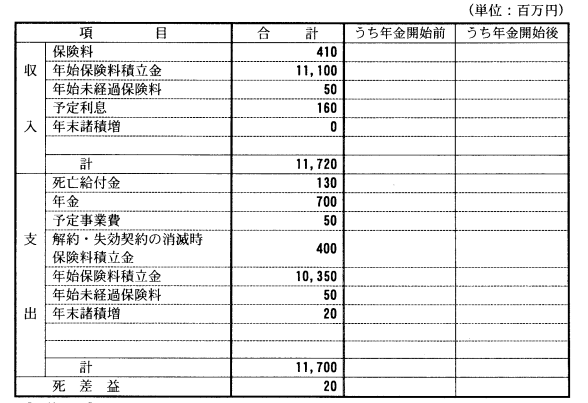
\includegraphics[scale=0.8]{./images/ProbH15-2-2-3-Shisaeki.png}\\

③死差益の計算(年金開始前と年金開始後の内訳)

\includegraphics[scale=0.8]{../../images/0886e4b052ffdfaa063a3b15de5a1a63b73379eb81154cbeb1e913a2fbbfc547.png}

\problem{H16 生保2問題 1(1)(2)
【一部記載変更】}

(1) 以下の表は生命保険会社の損益計算書の一部である。以下の空欄を適当な語句で埋めよ。

\includegraphics{../../images/41c5a6d4c389ed60ea4faf2f5511d3e737a20dfe474c939333f2cf9d19045085.png}

(2) 上記の損益計算書において、その他計上費用の内訳として計算される「税金」に含まれる税金の名称を5つ挙げよ。

\answer{解答}

(1) )①保険料等収入②保険金等支払金③支払備金④事業費⑤経常利益

(2) その他経常費用の内訳に入る税金

(消費税、印紙税、登録免許税、地方消費税、法人事業税、固定資産税、不動産取得税、事業所税などの中から5つを解答)

[法人税、住民税は「その他経常費用」ではないため誤り]


\problem{H13 生保2問題1(9)}

平成 12年度決算より生命保険会社に「基礎利益」の計算が義務付けられたが「基礎利益」について簡潔に説明せよ。

\answer{解答}

\begin{itemize}
\tightlist
\item
  基礎利益は、

  \begin{itemize}
  \tightlist
  \item
    保険業務や運用業務といった生命保険金杜の本業で得た利益を示すもので、
  \item
    「経常利益」から、

    \begin{itemize}
    \tightlist
    \item
      金融市場の変動に影響される損益である有価証券売却損益・有価証券評価損等の「キャピタル損益」、および、
    \item
      危険準備金繰入(戻入)額・個別貸倒引当金繰入額等の「臨時損益」を控除して計算する。
    \end{itemize}
  \end{itemize}
\end{itemize}

\begin{center}\rule{0.5\linewidth}{0.5pt}\end{center}

\subsection{配当準備金}

\problem{H24 生保2問題
1(2)}

生命保険相互会社における剰余金の分配に関し、以下の①~⑤の空欄に当てはまる適切な語句を記入しなさい。

\begin{itemize}
 \item 保険業法第 55 条の 2 では「剰余金の分配は、
 ①な分配をするための基準として内閣府令で定める基準に従い、行わなければならない。」と定めている。「内閣府令で定める基準」として、保険業法施行規則第
 30 条の 2 で以下のとおり規定している。
 \item 相互会社が社員に対する剰余金の分配をする場合には、②に応じて設定した区分ごとに、剰余金の分配の対象となる金額を計算し、次の各号に掲げるいずかの方法により、又はそれらの方法の併用により行わなければならない。
\end{itemize}
\begin{enumerate}
 \item 
 社員が支払った保険料及び保険料として収受した金銭を運用することによって得られる収益から、保険金、返戻金その他の給付金の支払、事業費の支出その他の費用等を控除した金額に応じて分配する方法(③方式)
 \item 
 剰余金の分配の対象となる金額をその発生の原因ごとに把握し、それぞれ各保険契約の責任準備金、保険金その他の基準となる金額に応じで計算し、その合計額を分配する方法(④方式)
 \item 剰余金の分配の対象となる金額を⑤等により把握し、各保険契約の責任準備金、保険料その他の基準となる金額に応じて計算した金額を分配する方法
 \item その他前三号に掲げる方法に準ずる方法
\end{enumerate}

\answer{解答}

①公正かつ衡平, ②保険契約の特性, ③アセット・シェア, ④利源別配当,
⑤保険期間

\problem{H11 生保2問題1(7)}

次の①~⑤を適当な語句で埋めよ。

保険業法施行規則第 25 条(現在は、30条の2)に定める剰余金の分配をする場合には、保険契約の①に応じて設定した区分ごとに、剰余金の分配の対象となる金額を計算し、次のいずれかの方法、またはそれらの方法の併用により行われなければならない。

\begin{enumerate}
 \item [一 ]
 社員が支払った保険料及び保険料として収受した金銭を運用することによって得られる収益から、保険金、返戻金その他の給付金の支払、事業費の支出その他の費用等を控除した金額に応じて分配する方法
 \item [二 ]
 剰余金の分配の対象となる金額をその発生の②ごとに把握し、それぞれ各保険契約の③・保険金その他の基準となる金額に応じて計算し、その合計額を分配する方法
 \item [三 ]
 剰余金の分配の対象となる金額を④等により把握し、各保険契約の⑤、保険料その他の基準となる金額に応じて計算した金額を分配する方法
 \item  [四 ] その他前三号に掲げる方法に準ずる方法
\end{enumerate}

\answer{解答}

①特性(商品特性等も可)②原因(利源等も可)
③責任準備金④保険期間⑤責任準備金

\problem{2019 生保2問題1(2)④改題}

生命保険会計に関する以下の文章について、下線場合は×を記入するとともに下線部分が正しい場合は〇を記入し、誤っている部分を正しい内容に改めなさい。

④
契約者(社員)配当準備金の積立限度は、積立配当の額、未払配当の額、\underline{翌期配当所要額}およびこれらに準ずるものとして保険料及び責任準備金の算出方法書において定める額の合計額である。

\answer{解答}

× 全件消滅時配当の額

\problem{H21 生保2問題1(2)}

生命保険相互会社の社員配当準備金に関し、次の①~⑤の空欄に当てはまる最も適切な語句を記入しなさい。

社員配当準備金は、保険業法施行規則により、その上限が次の合計額とされている。
\begin{itemize}
 \item ①の額 
 \item ②の額(決算期においては③を含む。) 
 \item ④の額
 \item その他上記に準ずるものとして保険料及び責任準備金の算出方法書に定める方法により計算した額
\end{itemize}

税法上の社員配当準備金繰入額の損金算入限度額は、②の額のうちの③である。

なお、社員配当準備金を超えて積み立てるものとしては、純資産の部に計上する⑤が規定されている。

\answer{解答}

①積立配当, ②未払配当, ③翌期配当所要額, ④全件消滅時配当,
⑤社員配当平衡積立金


\problem{H10 生保2問題
1(5)}

次の①~⑤を適当な語句で埋めよ。

保険業法施行規則第 28 条(現在、第 30
条の5)に定める社員配当準備金の限度額は、
①の額、②の額、③の額、④において定める額の合計額であり、決算期においては、②の額に⑤に分配する予定の配当の額が含まれる。

\answer{解答}

①積立配当(全件消滅時配当)、②未払配当、③全件消滅時配当(積立配当)、④算出方法書、⑤翌期


\problem{H16 生保2問題
1(6)}

社員(契約者)配当準備金の積立限度について簡潔に説明せよ。

\answer{解答}

社員配当準備金は、社員に対する剰余金の分配をするための準備金として、保険業法第58条第2項に定められている準備金の一つである。社員配当準備金は、平成8年に施行された現在の保険業法では以下に定める上限が設定され、負債の部に積み立てることとされた。これを超えて積み立てるものとしては資本の部に積み立てる社員配当平衡積立金が規定されている。
この社員配当準備金の上限は、保険業法施行規則第28条によれば、以下の合計額とされている。
\begin{enumerate}
\item [①] 積立配当(社員に分配された配当で利息を付して積み立てているものをいう。)の額
\item [②] 未払配当(社員に分配された配当で支払われていないもののうち、①で規定する積立配当以外のものをいう。)の額(決算期においては、翌期に分配する予定の配当の額を含む)
\item [③] 全件消滅時配当(保険契約の全てが消滅したと仮定して計算した当該保険契約の消滅時に支払う配当をいう。)の額
\item [④] その他前三号に掲げるものに準ずるものとして、保険料及び責任準備金の算出方法書において定める方法により計算した金額
\end{enumerate}

[上記は、相互会社における社員配当準備金の場合の解答例である。]

\problem{H10 生保2問題1(4)}

次の①~⑤を適当な語句で埋めよ。 

保険業法施行規則第 27 条(現在、第 30条の4)に定める剰余金の処分の対象となる金額は、当期末処分剰余金の額より次の(ⅰ)から(ⅴ)の合計額を控除した金額である。

\begin{enumerate} [(i) ]
\item ①の額 
\item ②目的取崩額 
\item ③の支払額
\item ④および基金償却積立金としてその決算期に積み立てる額 
\item 保険業法第59 条第 1 項において準用する商法 286 条ノ 3の規定により貸借対照表の⑤の部に計上した金額
\end{enumerate}

\answer{解答}

①前期繰越剰余金、②任意積立金、③基金利息、④損失てん補準備金、⑤資産

\problem{H1 生保2問題
2(2)}

「社員配当準備金明細表」における、前年度末から当年度末に係る異動状況について、「前年度末残高」「前年度剰余金からの繰入額」「利息による増加額」「支払いによる減少額」の各項目を説明せよ。

\answer{解答}

社員配当準備金明細表は、期中にあける同準備金の異動状況を表わしており、次の関係が成り立つ。

「前年度末残高」+「前年度剰余金からの繰入額」+「利息による増加」-「支払による減少」(±「その他による増減額」)=「当年度末残高」

各項目の内容は次の通りである。

「前年度末残高」 前年度末における配当準備金の残高で、前年度の貸借対照表の配当準備一金の金額である。内訳は、割当済未払のもの、積立・据置中のもの等(その他はたまり)である。

「前年度剰余金からの繰入額」 前年度の剰余金処分により配当準備金に繰り入れた金額であり、定款においては、剰余金の90%以上を繰り入れることとしている。
{更に、翌期所要額までは無税繰入という税法限度について言及することも解答もあった。}

「利息による増加額」 積立配当金の利息による増加分である。
{更に、当期の損益計算書の「社員配当金」と「社員配当準備金戻入額」の差額と一致する関係にあることを述べる解答もあった。}

「支払による減少」 当期において社員配当金として支払処理された金額であり、損益計算書の「社費配当金」の金額と一致する。
{以上に加え、生保特有の配当準備金を巡る会計処理の諸問題について論じる解答もあった。}

\problem{H2 生保2問題
3(1)改}

契約者配当準備金に関し、いわゆる「たまり」の発生メカニズムについて説明せよ。

\problem{H2 生保2問題
3(1)改}

解答のポイントとしては、\\
・法人税法上の取扱いについては、税法上の損金繰入れ限度について述べ、同時に洗い替えによる「たまり」の益金算入について述べること。また、過去の繰入眼度についてと、その考え方についても述べれば更に良い。

「たまり」発生のメカニズムについては、\\
・配当準備金に翌期配当所要額を超えて繰入れた場合、応答日前の解約失効による消滅にともなう発生の場合等について述べる。

「たまり」の意義についての所見は、\\
・税法上は「たまり」の損金扱いは認められないが、生命保険配当の仕組みから配当準備金の計理上、また経営上からも必要であること、さらにその帰属、還元等についてふれると良い。

(解答例)

・生命保険会社における契約者配当準備金に関しての法人税法上の取扱いは次のとおり。
\begin{enumerate} [1) ]
\item 昭和51年以前は、損金算入繰入限度額は普通保険では、3年目配当方式の考え方、団体保険では、2年目配当方式の考え方に基づき、普通保険は、翌期配当所要額と翌々期配当所要額の和半、団体保険では、翌期配当所要額となっていたが現在は、
\item 翌期配当所要額が繰入れ限度額で、また洗い替え方式が導入されている。
\end{enumerate}

「たまり」の発生のメカニズムの主なものは、
\begin{enumerate} [1) ]
\item 翌期配当所要額は事業年度末有効契約に対して計上するが、一方、応答日前の解約・失効については、配当は支払われないため「たまり」が発生する。
\item 2年目配当においては、翌期配当所要額を推定計算すること、また転換契約にともなう配当所要額も推定計算によっているため、「たまり」発生の原因となる。勿論この場合は「たまり」が負になることもある。
\item 翌期配当所要額を超えて繰入れた場合も、「たまり」が発生する。
\end{enumerate}

翌期配当所要額に満たない繰入れをする場合もあるので、毎年必ず発生するわけではない。

以上まとめると、「たまり」の種類としては次の3種類が考えられる。

「新たまり」 翌期配当所要額を配当準備金に繰入れるが、約款の規定等により配当未払が生じたことによる「たまり」

「翌期超」 翌期配当所要額を超えて繰入れたことにより発生する「たまり」

「過年度分」 過去の「新たまり」「翌期超」のうち現在配当準備金の中に残っている部分

これらの「たまり」の使用こついては、従来より「たまり」を取崩す(決算上は翌期配当所要額に満たない繰入れ)こともあったが、「たまり」については帰属が明確でなく、その経理方法に関しても問題あるとの意見があり、「たまり」の位置付け、経理方法を検討する必要が出てきている。
一方、翌期配当所要額を繰入れている限りは、毎年「たまり」が発生し配当準備金中に累積され、いわゆる内部留保を形成することになる。

「たまり」は以下の理由により必要と考えられている。
\begin{enumerate}[ 1) ]
\item 生命保険の配当の大部分が3年目配当となっていることを考えれば、事業年度末において剰余金を配当準備金に繰入れる場合、剰余と配当の対応をとれば(翌期配当所要額+翌々期配当所要額)×1/2が必要となり、法人税法での前提である「配当準備金の年度末の積立額は翌期配当所要額の水準」では充分とはいえない。望ましい配当準備金の額は、翌期配当所要額+1/2翌々期配当所要額が基準となる。従って、一定レベルの「たまり」は必要である。
\item 生命保険の配当は従来より、経営実績を反映しつつも、ある程度安定的に行われており、契約者にも受入れられている。従って、安定配当財源として、「たまり」を配当準備金に積立てておくことは必要である。いわば、平衡準備金としての機能を必要とする。
\end{enumerate}

一方、以上の状況から「たまり」は必要だからといっても無制限という訳にはいかない。契約者への還元を考えれば、そこには一定のルールが必要である。配当準備金の負債性を考えた場合、または平衡準備金としての性格を考えた場合、経営のバッファーとして考えた場合等、そこには検討すべき事が多い。その際には「たまり」の発生は繰入額にも原因がある訳で、繰入額の計算方法(2年目配当、特別配当を含む)を同時に検討をする必要がある。

所見について(各自の考え方を述べる)例えば、
\begin{enumerate}
\item 積極的にその意義を認め、さらに帰属性を考慮し、還元すべきか否か、また還元するとした場合その方法について述べる。あるいは、
\item 「たまり」は解約・失効のように割当て未分配によるもの、未割当繰入によるものも考えられるが、前者については、契約者に対する公平性を考えた場合、未分配となる現状の割当て規定で良いのか、また後者については、その是非を述べる。さらに、
\item 保険審議会の検討項目である「広義の自己資本」にからめて述べるのもよい
\end{enumerate}

\problem{H18 生保2問題
1(1)}

相互会社における事業年度末の社員配当準備金明細表及び社員配当準備金・社員配当金の経理処理に関し、以下の空欄を埋めよ。

社員配当準備金明細表

\begin{tabularx}{\textwidth}{|X|r|X|}
\hline
項目 & 金額 & 摘要\\ \hline
前年度末現在高 & 3,000 & ・前年度末積立配当金・①配当金等\\ 
②からの繰入額 & 3,500 &\\ 
利息による増加額 & 100 & ・積立配当金の利息による増加\\ 
支払による減少額 & 3,200 &\\ 
その他による増減額 & 0 &\\ 
当年度末現在高 & 3,400 &\\ \hline
\end{tabularx}
\\\\

\begin{tabularx}{\linewidth}{Xr|Xr}
\multicolumn{4}{l} {上記明細表に基づく③の支払に係る仕訳(注)}\\
\hline
④ & 3,200& ③ & 3,200\\
\end{tabularx}
\\\\


\begin{tabularx}{\linewidth}{Xr|Xr}
\multicolumn{4}{l} {積立配当金のうち利息により増加した部分に係る仕訳}\\
\hline
⑤ & 100& ④ & 100\\
\end{tabularx}
\\\\

(注)期中に③として支払い処理した金額の合計額に対応する処理である。なお、期中の③の支払いを④の減少で処理している会社にあっては、この振替処理は不要である。

\answer{解答}

①  未払, ②  前年度剰余, ③  社員配当金, ④  社員配当準備金, ⑤  積立配当金積立利息繰入額

\problem{H13 生保2問題
1(7)}

生命保険相互会社は、剰余の
80%以上を内閣府令に定める準備金に繰り入れなければならないとされている。次の生命保険相互会社の剰余金処分決議書から、当該会社の配当還元率を計算しなさい。(解答は%表示とし、小数点以下第2 位を四捨五入して、小数点以下第 1
位まで求めよ。)なお、その計算過程についても記載すること。

\includegraphics[scale=.8]{../../images/6494e79c67c53af6e1c861f5fac61fcc619faf0b31f01c3983095ead5402b351.png}

\answer{解答}

保険業法第58条第2項および施行規則第27条・第28条の規定により計算する。

分子:社員配当準備金35,000+社員配当平衡積立金3,100=38,100百万円

分母:当期未処分剰余金100,000-前期繰越剰余金45,000-損失てん補準備金200-基金利息1,200-基金償却準備金10,000=43,600百万円

したがって、配当還元率=38,100÷43,600=87.4%(答)

\begin{center}\rule{0.5\linewidth}{0.5pt}\end{center}

\section{1.7
生命保険会社税制}

\problem{H26 生保2問題
1(4)}

生命保険会社の法人税課税について、次の空欄を埋めなさい。
\begin{itemize}
\item 責任準備金繰入額については、保険料積立金及び未経過保険料の部分に限り、算出方法書に定められている①を基として計算した額を限度として損金算入できる。保険料積立金については②で計算した額を限度とする。ただし、標準責任準備金の対象契約については、平成8 年の大蔵省告示第 48号に定められた計算基礎率により計算した額を損金算入限度額とすることができる。
\item 7\%最低課税方式とは、③が当期剰余金の7\%相当額に満たない場合は、剰余金の7\%相当額をもって課税標準とする方式である。ただし、④、心身障害者扶養者生命保険、再保険に係る剰余金は2 分の 1 に減額して計算する。
\item 契約者(社員)配当準備金繰入額の損金処理が認められている。ただし、⑤が上限とされている。
\end{itemize}

\answer{解答}

① 保険料の計算基礎, ② 平準純保険料式, ③ 課税所得, ④ 団体定期保険, ⑤
翌期配当所要額

\begin{center}\rule{0.5\linewidth}{0.5pt}\end{center}

\problem{H23 生保2問題
1(3)}

生命保険会社に特有の税制に関し、以下の①~⑤の空欄に当てはまる適切な語句を記入しなさい。
\begin{itemize}
 \item 課税所得が当該事業年度の①の額の 7%相当額に満たない場合は、この7%相当額を課税標準とする。ただし、団体定期保険、心身障害者扶養者生命保険、再保険に係る①は2 分の 1 に減額している。
 \item 法人株主が株式の配当金を受け取った場合、法人間の②を排除するため、法人税法上、受取配当金等の一部について益金不算入が認められている。しかし、生命保険会社が受取配当金等の益金不算入を適用する場合には、益金不算入とした金額が③の損金算入限度から控除されるため、実質的には受取配当金等の益金不算入の恩恵を受けることができない。
 \item 法人事業税の課税標準は、収入保険料中の④相当額とするとの考え方から、収入保険料に一定割合を乗じた金額と定められている。なお、平成20 年 10 月 1日以降に開始する事業年度から法人事業税の税率を引き下げるとともに、⑤が創設されている。
\end{itemize}

\answer{解答}

① 剰余金  ② 二重課税 ③ 配当準備金 ④ 付加保険料 ⑤ 地方法人特別税


\problem{H13 生保2問題
1(4)}

生命保険会社の法人税課税について、次の①~⑤を適当な語句で埋めよ。
\begin{enumerate} [(a) ]
\item 7%最低課税方式とは、課税所得が当期①の
 7%相当額に満たない場合は、①の7%相当額をもって②とする方式である。ただし、
 ③、心身障害者扶養者生命保険、再保険に係る①は 2 分の 1
 に減額して計算する。 
\item 責任準備金の繰入額については、
 ④で計算した積立額を限度として、損金算入が認められている。
 \item 
契約者配当準備金繰入額の損金処理が認められている。ただし、⑤が上限とされている。
\end{enumerate}

\answer{解答}

①  剰余金 ②   課税標準 ③   団体定期保険  ④ (平準)純保険料式  ⑤   翌期配当所要額

\problem{H8 生保2問題 1(2)、H1 生保2問題 1(3)}
7%課税方式について、最近の状況も踏まえ説明せよ。

\answer{解答}
課税所得が当期剰余金の7%相当額に満たない場合は、剰余金の7%相当額をもって課税標準とする方法。ただし、団体定期保険、心身障害者保険、再保険に係る剰余金は2分の1に減額して計算することになっている。
純保険料式資任準備金を達成する以前は、この方式に該当する会社が多かったが、最近は、業績状況の低迷等により課税所得が減少して該当する場合が生じている。\strut

\problem{H4 生保2問題 1(3)、H2 生保2問題3(1)}

法人税法上の契約者配当準備金繰入限度額について簡潔に説明せよ。

\answer{解答}

契約者配当準備金繰入額については、昭和52年3月決算期から翌朝配当所要額を限度に損金算入が認められている。
それ以前は、3年目配当の保険種類については(翌朝配当所要額+翌々期配当所要額)/2が損金算入限度であった。


\problem{H3 生保2問題
2(1)}

受取配当金の法人税法上の取扱について、一般事業会社と生命保険会社の相違点を説明せよ。


\answer{解答}

一般事業会社においては、法人株主が配当金を受け取った場合、すでに配当金を支払う法人の段階で、法人税が課税されているので、法人間の2重課税を排除するため、法人税法上受取配当金の益金不算入が認められている。
これに対して、生命保険会社の場合は、原則として翌朝配当所要額を限度として契約者配当準備金繰入額は損金処理が認められており、受取配当金の益金不算入を行った時は、相当する金額だけ契約者配当準備金の損金算入を否認されるため、実質は受取配当金等の益金不算入の適用が除外されていることになる。

\problem{H15 生保2問題
1(2)}

日本における生命保険会社の法人事業税に関し、次の①~⑤について、正しいものには○、誤っているものには×を付けよ。
\begin{enumerate}
\item[①] 法人事業税は地方税法に基づく税である。
\item[②] 生命保険業の収入金額は、個人保険のうち貯蓄保険以外については、各事業年度の収入保険料に100分の 24 を乗じて得た金額である。
\item[③] 個人保険のうち貯蓄保険は、保険期間が 5年以下で所定の保険金額を支払う定めのある生命保険である。
\item[④] 生命保険事業について収入金額の算定で、収入保険料のうち未収保険料および未経過保険料はその事業年度の収入とならない。
\item[⑤] 生命保険業を行う法人の標準税率は、収入金額の 1.5%である。
\end{enumerate}

\answer{解答}

①○ ②○ ③×[5年以下→10年以下]
④×[未経過保険料はその事業年度の収入となる] ⑤×[1.5%→1.3%]

\begin{center}\rule{0.5\linewidth}{0.5pt}\end{center}

\problem{H12 生保2問題 1(10)、H7 生保2問題 1(4)、H2 生保2問題
1(4)}

生命保険会社の法人事業税について簡潔に説明せよ。

\answer{解答}

\begin{itemize}
\tightlist
\item
  法人事業税は法人の行う事業に対し、その法人に課せられる地方税である。
\item
  生命保険業にあっては各事業年度の収入金額が課税標準となり、その収入金額は保険種類ごとに保険料収入の一定率となっている。
\item
  収入金額の算定は保険料が現実に収入された事業年度によって行なわれ、税率1.3/100(改正前1.5/100)となっている。
\end{itemize}

\end{document}
